\documentclass[oneside,a4paper]{extreport}

% !TeX root = ../main.tex

\usepackage{fontspec}
\usepackage{polyglossia}
\setmainlanguage{vietnamese}
\setotherlanguages{english}
\setmainfont{Times New Roman}
\fontsize{13pt}{15.6pt}\selectfont % 13pt font with 1.2 line spacing

\usepackage{url}

\usepackage{listings}
\usepackage[dvipsnames]{xcolor}
\lstdefinelanguage{Go}{
    morekeywords={break,case,chan,const,continue,default,defer,else,
            fallthrough,for,func,go,goto,if,import,interface,map,package,range,
            return,select,struct,switch,type,var,nil,true,false,iota},
    sensitive=true,
    morecomment=[l]{//},
    morecomment=[s]{/*}{*/},
    morestring=[b]",
}

\lstset{
    language=Go,
    basicstyle=\ttfamily\footnotesize,
    keywordstyle=\color{blue!80!black}\bfseries,
    commentstyle=\color{gray}\itshape,
    stringstyle=\color{red!70!black},
    numbers=left,
    numberstyle=\tiny\color{gray},
    stepnumber=1,
    numbersep=10pt,
    showstringspaces=false,
    tabsize=2,
    breaklines=true,
    backgroundcolor=\color{gray!5},
    frame=single,
    captionpos=b
}

\newcommand\YAMLcolonstyle{\color{red}\mdseries}
\newcommand\YAMLkeystyle{\color{black}\bfseries}
\newcommand\YAMLvaluestyle{\color{blue}\mdseries}

\makeatletter

% here is a macro expanding to the name of the language
% (handy if you decide to change it further down the road)
\newcommand\language@yaml{yaml}

\expandafter\expandafter\expandafter\lstdefinelanguage
\expandafter{\language@yaml}
{
keywords={true,false,null,y,n},
keywordstyle=\color{darkgray}\bfseries,
basicstyle=\YAMLkeystyle,                                 % assuming a key comes first
sensitive=false,
comment=[l]{\#},
morecomment=[s]{/*}{*/},
commentstyle=\color{purple}\ttfamily,
stringstyle=\YAMLvaluestyle\ttfamily,
moredelim=[l][\color{orange}]{\&},
moredelim=[l][\color{magenta}]{*},
moredelim=**[il][\YAMLcolonstyle{:}\YAMLvaluestyle]{:},   % switch to value style at :
morestring=[b]',
morestring=[b]",
literate =    {---}{{\ProcessThreeDashes}}3
{>}{{\textcolor{red}\textgreater}}1
{|}{{\textcolor{red}\textbar}}1
{\ -\ }{{\mdseries\ -\ }}3,
}

% switch to key style at EOL
\lst@AddToHook{EveryLine}{\ifx\lst@language\language@yaml\YAMLkeystyle\fi}
\makeatother

\newcommand\ProcessThreeDashes{\llap{\color{cyan}\mdseries-{-}-}}
\usepackage{listings}

\lstdefinelanguage{HCL}{
    keywords={resource, data, provider, module, variable, output, locals, terraform, required_providers, backend, provisioner, depends_on, count, for_each, if, each, sensitive, type, default, description},
    keywordstyle=\color{blue}\bfseries,
    ndkeywords={true, false, null},
    ndkeywordstyle=\color{magenta}\bfseries,
    identifierstyle=\color{black},
    commentstyle=\color{gray}\textit,
    stringstyle=\color{red},
    numbers=left,
    numberstyle=\scriptsize\color{black},
    stepnumber=1,
    numbersep=8pt,
    breaklines=true,
    breakatwhitespace=true,
    tabsize=2,
    basicstyle=\ttfamily\footnotesize,
    moredelim=[is][\color{darkgray}]{<<}{>>}, % For custom delimiters if needed
    moredelim=[l][\color{ForestGreen}]{//},    % For single-line comments
    moredelim=[s][\color{ForestGreen}]{/*}{*/}, % For multi-line comments
}

\usepackage{svg}
\usepackage{graphicx}
\graphicspath{{./images/}{./topologies/images/}}
\usepackage[export]{adjustbox}
\usepackage{float}
\usepackage{booktabs}

% Tài liệu tham khảo
\usepackage[
    sorting=nty,
    backend=biber,
    language=english,
    % backend=bibtex,
    defernumbers=true]{biblatex}
\usepackage[unicode]{hyperref} % Bookmark tiếng Việt
% Override biblatex strings with Vietnamese
\DefineBibliographyStrings{english}{
    bibliography = {Tài liệu tham khảo},
    references   = {Tài liệu tham khảo},
    and          = {và},
    in           = {trong},
    editor       = {Biên tập},
    editors      = {Biên tập},
    translator   = {Dịch giả},
    page         = {trang},
    pages        = {trang},
    volume       = {tập},
    number       = {số},
    % journal      = {Tạp chí},
    urlseen      = {truy cập ngày},
    % online       = {Trực tuyến},
    % date         = {ngày},
    edition      = {ấn bản},
}
\addbibresource{references.bib}

% Đổi tên mặc định
\renewcommand{\chaptername}{Chương}
\renewcommand{\figurename}{Hình}
\renewcommand{\tablename}{Bảng}
\renewcommand{\contentsname}{Mục lục}
\renewcommand{\listfigurename}{Danh sách hình}
\renewcommand{\listtablename}{Danh sách bảng}
\renewcommand{\appendixname}{Phụ lục}

% Định dạng chapter
\usepackage{titlesec}
\titleformat{\chapter}
[display]
{\normalfont\bfseries\large}{\chaptername \ \thechapter}{10pt}{\huge}
\titlespacing*{\chapter}{0pt}{-10pt}{20pt} %khoảng cách giữa chapter và đầu trang

\titleformat{\section}
{\normalfont\bfseries\large}{\thesection}{1em}{}

\titleformat{\subsection}
{\normalfont\bfseries\normalsize}{\thesubsection}{1em}{}

\usepackage{geometry} % For setting page margins
\usepackage{setspace} % For adjusting line spacing
\usepackage{parskip} % For setting paragraph spacing
\usepackage{indentfirst} % For indenting the first line of a paragraph

% --- Page Margins ---
\geometry{
    top=2.5cm,
    bottom=3cm,
    left=3cm,
    right=2cm,
}

% --- Line Spacing ---
\linespread{1.3} % Equivalent to 1.3 lines spacing

% --- Paragraph Spacing ---
\setlength{\parskip}{6pt plus 0pt minus 0pt} % 6pt spacing between paragraphs

% --- Paragraph Indentation ---
\setlength{\parindent}{1cm} % 1cm indentation for the first line of each paragraph

% Trang bìa
\usepackage{tikz}
\usetikzlibrary{calc}
\newcommand\HRule{\rule{\textwidth}{1pt}}

\usepackage{hyperref}

\usepackage{amsmath}
\usepackage{amssymb}

% ========================================================================================= %
% CHÚ Ý: Thông tin chung về KLTN - sinh viên điền vào đây để tự động update các trang khác  %
% ========================================================================================= %
\newcommand{\tenSV}{Lương~Nhật~Hào} % Dấu ~ là khoảng trắng không được tách (các chữ nối với nhau bằng dấu ~ sẽ nằm cùng 1 dòng
\newcommand{\mssv}{21020196}
\newcommand{\tenKL}{Sử~dụng~LaTeX trong Khoá~luận~tốt~nghiệp} % Chú ý dấu ~ trong tên khóa luận
\newcommand{\tenGVHD}{Phạm~Mạnh~Linh}
\newcommand{\tenBM}{Công~nghệ~thông~tin-Mạng~máy~tính}
\begin{document}

% \fontfamily{phv}\selectfont

\begin{titlepage}
    \begin{tikzpicture}[remember picture, overlay]
        \draw[line width=3pt]
        ($ (current page.north west) + (1cm,-1cm) $)
        rectangle
        ($ (current page.south east) + (-1cm,1cm) $);
    \end{tikzpicture}
    \begin{center}
        {
            \textbf{\fontsize{12}{14.4}\selectfont{ĐẠI HỌC QUỐC GIA HÀ NỘI\\
                    TRƯỜNG ĐẠI HỌC CÔNG NGHỆ}}\\
        }
        \vspace{1cm}
        
\includegraphics{logo-uet.png}\\
        \textbf{\fontsize{14}{16.8}\selectfont{\tenSV}}\\
        \vspace{1.5cm}
        \textbf{\fontsize{18}{21.6}\selectfont{{\tenKLU}}}\\
        \vspace{1cm}
        \textbf{\fontsize{14}{16.8}\selectfont{ĐỒ ÁN TỐT NGHIỆP ĐẠI HỌC HỆ CHÍNH QUY}}\\
        \textbf{\fontsize{14}{16.8}\selectfont{Ngành: Mạng máy tính và truyền thông dữ liệu}}
        \vfill
        \noindent\textbf{\fontsize{12}{14.4}\selectfont{HÀ NỘI - 2025}}
    \end{center}
\end{titlepage}
\begin{titlepage}
    \begin{tikzpicture}[remember picture, overlay]
        \draw[line width=2pt]
        ($ (current page.north west) + (1cm,-1cm) $)
        rectangle
        ($ (current page.south east) + (-1cm,1cm) $);
    \end{tikzpicture}
    \begin{center}
        {
            \textbf{\fontsize{12}{14.4}\selectfont{ĐẠI HỌC QUỐC GIA HÀ NỘI\\
                    TRƯỜNG ĐẠI HỌC CÔNG NGHỆ}}\\
        }
        \vspace{1cm}
        \textbf{\fontsize{14}{16.8}\selectfont{Lương Nhật Hào}}\\
        \vspace{1.5cm}
        \textbf{\fontsize{18}{21.6}\selectfont{{NGHIÊN CỨU KĨ THUẬT CO GIÃN TÀI NGUYÊN ĐA CẤP ĐỘ CHỦ ĐỘNG CHO ỨNG DỤNG SMARTHOME TRONG MÔI TRƯỜNG ĐIỆN TOÁN ĐÁM MÂY}}}\\
        \vspace{1cm}
        \textbf{\fontsize{14}{16.8}\selectfont{ĐỒ ÁN TỐT NGHIỆP ĐẠI HỌC HỆ CHÍNH QUY}}\\
        \textbf{\fontsize{14}{16.8}\selectfont{Ngành: Mạng máy tính và truyền thông dữ liệu}}

        \vfill

        \raggedright
        \textbf{\fontsize{14}{16.8}\selectfont{Cán bộ hướng dẫn: Phạm Mạnh Linh}} \\
        \vspace{3cm}
        \textbf{\fontsize{14}{16.8}\selectfont{Cán bộ đồng hướng dẫn: Trần Anh Tú}}

        \vfill

        \centering
        \noindent\textbf{\fontsize{12}{14.4}\selectfont{HÀ NỘI - 25}}
    \end{center}
\end{titlepage}


% Mục lục, danh sách hình, danh sách bảng
\addcontentsline{toc}{chapter}{Mục lục}
\tableofcontents
\listoffigures
\listoftables

\begin{titlepage}
  \addcontentsline{toc}{chapter}{TÓM TẮT}
  \begin{center}
    \textbf{\fontsize{12}{14.4}\selectfont{TÓM TẮT}}
  \end{center}

  \fontsize{12}{14.4}\selectfont{
    Hiện nay
  }

  \noindent\textbf{Từ khóa}: Điện toán đám mây, Co dãn chủ động, Nhà thông minh.

  \newpage

  \addcontentsline{toc}{chapter}{Lời cảm ơn}
  \begin{center}
    \textbf{\fontsize{12}{14.4}\selectfont\uppercase{{Lời cảm ơn}}}
  \end{center}

  Lời đầu tiên, em xin bày tỏ lòng biết ơn sâu sắc đến giảng viên hướng dẫn - TS.Phạm Mạnh Linh, người đã tận tình hướng dẫn, chỉ bảo và truyền đạt những kiến thức quý báu trong suốt quá trình em thực hiện đồ án này. Đồng thời, em cũng xin cảm ơn giảng viên đồng hướng dẫn - Ths. Trần Anh Tú đã chỉ hướng, giải đáp, hỗ trợ em giúp em vượt qua những khó khăn trong việc nghiên cứu và hoàn thiện đồ án một cách tốt nhất.

  Em cũng xin chân thành cảm ơn các thầy, cô cùng bạn bè trong khoa Mạng máy tính và trường Đại học Công nghệ - Đại học Quốc gia Hà Nội đã tạo điều kiện về cơ sở vật chất, trang thiết bị và môi trường học tập lý tưởng để em có thể nghiên cứu và thực hiện đồ án này cũng như hướng dẫn, chỉ bảo em trong suốt thời gian học tập tại trường.

  Cuối cùng, em xin gửi lời cảm ơn đến bạn bè, đồng nghiệp, người thân vì sự hỗ trợ nhiệt tình, những ý kiến đóng góp quý báu kèm với sự động viên tinh thân vô cùng to lớn mà họ đã dành cho em trong suốt thời gian qua.

  \begin{flushright}
    \begin{minipage}{0.6\linewidth}
      \begin{center}
        Hà Nội, ngày  tháng  năm 2025\\
        Sinh viên\\
        \vspace{2cm}
        Lương Nhật Hào
      \end{center}
    \end{minipage}
  \end{flushright}

  % Abbreviation
  % public cloud
  % CI/CD
\end{titlepage}
\chapter{Mở đầu}

\section{Đặt vấn đề}

Trong bối cảnh hiện nay, khi tốc độ chuyển đổi số đang rất nhanh và không ngừng gia tăng, khi các thiết bị, vật dụng hằng ngày không ngừng được cải tiến, nâng cấp để nâng cao trải nghiệm người dùng, thì những công nghệ như đồng hồ thông minh, đèn điện tự động, khóa cửa từ đang dần trở thành một phần tất yếu trong không gian sống của mỗi các nhân.

Mạng lưới tập hợp các thiết bị thông minh và công nghệ tạo điều kiện thuận lợi cho hoạt động giao tiếp giữa thiết bị và đám mây cũng như giữa các thiết bị với nhau hình thành nên một mạng lưới mang tên Internet of Things (IoT) hay còn gọi là Internet vạn vật - thứ góp phần kiến tạo nên một môi trường sống thông minh, tiện nghi và linh hoạt chưa từng có.

Các thiết bị này ngày nay không còn chỉ thực hiện các chức năng đơn lẻ mà thông qua khả năng thu thập dữ liệu dựa trên các cảm biến về môi trường xung quanh, chúng đã có thể hỗ trợ cải thiện hệ thống một cách chủ động, hệ quả là nâng cao chất lượng trải nghiệm người dùng.

% tiếp

Tuy nhiên, khả năng thu thập dữ liệu này cũng có mặt hạn chế nhất định. Trong đó, có thể kể đến chính là lượng dữ liệu được gửi liên tục về hệ thống theo thời gian thực, đòi hỏi phải được xử lý với tốc độ nhanh và độ chính xác cao. Đây thực sự là bài toán khó đối với các hệ thống xử lý dữ liệu từ khâu thiết kế, triển khai cho đến vận hành.

Nhiều hệ thống xử lý luồng dữ liệu thời gian thực, điển hình là Apache Storm vốn không hề được trang bị cơ chế tài nguyên linh hoạt. Điều này khiến cho việc quản lý và duy trì vận hành hệ thống một cách thủ công trở nên tốn kém, thiếu hiệu quả, và dễ xảy ra sai sót.

Từ đây, vấn đề được đặt ra là: Làm sao để hệ thống có khả năng co dãn linh hoạt, chủ động - vừa tối ưu tài nguyên, vừa đảm bảo hiệu năng ổn định - không chỉ ở thời điểm hiện tại mà còn thích ứng tốt trong tương lai khi cả quy mô hệ thống lẫn khối lượng dữ liệu đều sẽ tăng theo thời gian?

Trên cơ sở đó, nghiên cứu này đề xuất giải pháp về co giãn tài nguyên đa cấp độ theo hướng chủ động, đồng thời vẫn tận dụng các ưu điểm vượt trội về khả năng xử lý thời gian thực, khả năng chịu lỗi và đảm bảo dữ liệu của hệ thống SmartHome đã được triển khai trên nền tảng Apache Storm.
\chapter{Tổng quan về công nghệ và cơ sở lý thuyết}

Trong chương này, đồ án sẽ trình bày các công nghệ và khái niệm cơ bản liên quan đến việc xây dựng hệ thống co dãn tài nguyên và đồng thời mô tả những vấn đề còn tồn đọng cần phải giải quyết. Mục tiêu là cung cấp một cái nhìn tổng quan về các thành phần chính được sử dụng trong hệ thống, làm cơ sở cho việc triển khai và đánh giá trong các chương 3 và 4 tiếp theo.

Chương 2 sẽ trình bày các nội dung chính sau đây:
\begin{itemize}
    \item Internet of Things
    \item Apache Storm
    \item Docker
    \item Giám sát hệ thống (monitoring)
    \item Đám mây công cộng (public cloud)
    \item Công cụ quản lý cơ sở hạ tầng Terraform
    \item Các phương pháp mở rộng
    \item Học tăng cường Q-learning
\end{itemize}

\section{Internet of Things}

Internet of Things \gls{iot} (Mạng lưới Vạn vật kết nối) là một khái niệm mô tả một hệ sinh thái nơi các vật thể vật lý không chỉ có thể kết nối và giao tiếp với nhau qua internet, mà còn có khả năng thu thập và truyền tải thông tin. Những vật thể này bao gồm thiết bị điện tử, phương tiện giao thông, đồ gia dụng, và thậm chí là những vật thể được trang bị cảm biến, phần mềm và kết nối mạng. Trên cơ sở này, chúng có thể tự động thu thập và chia sẻ dữ liệu mà không cần sự can thiệp của con người. Điều này giúp tăng cường khả năng tự động hóa và quản lý thông minh trong các lĩnh vực như nhà thông minh, giao thông thông minh, và chăm sóc sức khỏe thông minh.

Ví dụ: Một chiếc máy giặt thông minh có thể kết nối với ứng dụng trên điện thoại để báo cho bạn biết khi nào cần thay màng lọc hoặc khi quá trình giặt hoàn tất, toàn bộ những hành động này đều dựa trên dữ liệu thu thập được từ các cảm biến bên trong máy, thông qua kết nối mạng gửi đến trung tâm xử lý và gửi thông báo về các thiết bị của người dùng.

Nhờ tiềm năng to lớn của mình, các ứng dụng của  trải dài trên nhiều lĩnh vực và các mặt của đời sống xã hội, có thể kể đến như:

\begin{itemize}
    \item Giám sát các điều kiện môi trường trong nông trại.
    \item Quản lý các mô hình giao thông với ô tô thông minh và các thiết bị tự hành thông minh khác.
    \item Kiểm soát các máy móc và quy trình trong nhà máy.
    \item Theo dõi tồn kho và các lô hàng trong kho.
\end{itemize}

\section{Apache Storm}

Apache Storm \autocite{apachestorm} là một nền tảng tính toán thời gian thực phân tán, mã nguồn mở, được thiết kế để xử lý các luồng dữ liệu liên tục. Nó cung cấp chức năng tương tự như Apache Hadoop nhưng được tối ưu hóa để luồng dữ liệu không giới hạn (unbounded streams of data), trong khi Hadoop xử lý dữ liệu theo lô (batch processing).

Apache Storm có sử dụng đơn giản, có thể được sử dụng bởi bất kỳ ngôn ngữ lập trình nào. Nhờ đó, Apache Storm có thể được áp dụng trong nhiều lĩnh vực, bao gồm: phân tích thời gian thực, học máy trực tuyến, tính toán liên tục, RPC phân tán, ETL và hơn thế nữa. Hệ thống này có khả năng xử lý dữ liệu với tốc độ cao, đạt hiệu suất trên một triệu bộ dữ liệu mỗi giây trên mỗi nút trong các thử nghiệm hiệu năng. Nó cũng cung cấp khả năng mở rộng, khả năng chịu lỗi và đảm bảo xử lý dữ liệu đồng thời cũng dễ cài đặt, triển khai và vận hành.

\subsection{Đôi nét về xử lý dữ liệu luồng}

Xử lý luồng (Stream Processing)\autocite{rivery_batch_vs_stream} là phương pháp xử lý và phân tích dữ liệu liên tục, nơi dữ liệu được thu thập và phân tích ngay khi nó được tạo ra. Nhờ vậy, nó cho phép phản ứng ngay lập tức với các thay đổi, một yêu cầu thiết yếu cho các tác vụ đòi hỏi phải đưa ra quyết định nhanh.

So sánh với xử lý theo lô (Batch Processing):
\begin{itemize}
    \item \textbf{Xử lý dữ liệu:}
          \begin{itemize}
              \item Xử lý luồng: Xử lý dữ liệu liên tục, không ngừng nghỉ.
              \item Xử lý theo lô: Xử lý dữ liệu theo từng khối lớn, được xác định trước.
          \end{itemize}
    \item \textbf{Thời gian xử lý:}
          \begin{itemize}
              \item Xử lý luồng: Xử lý diễn ra trong thời gian thực, ngay khi dữ liệu được tạo ra.
              \item Xử lý theo lô: Xử lý diễn ra theo lịch trình cố định, không phải lúc dữ liệu được tạo ra.
          \end{itemize}
    \item \textbf{Độ phức tạp:}
          \begin{itemize}
              \item Xử lý luồng: Thường phức tạp hơn do yêu cầu xử lý liên tục và khả năng xảy ra các vấn đề về tính nhất quán.
              \item Xử lý theo lô: Thường đơn giản hơn, do dữ liệu được xử lý theo từng khối đã xác định.
          \end{itemize}
    \item \textbf{Độ trễ:}
          \begin{itemize}
              \item Xử lý luồng: Độ trễ thấp, cung cấp thông tin chi tiết ngay lập tức.
              \item Xử lý theo lô: Độ trễ cao hơn, thông tin chi tiết không có ngay lập tức.
          \end{itemize}
\end{itemize}

Các trường hợp sử dụng của xử lý luồng:
\begin{itemize}
    \item \textbf{Phát hiện gian lận}: Xác định các giao dịch hoặc hoạt động bất thường trong thời gian thực.
    \item \textbf{Giám sát mạng}: Theo dõi lưu lượng mạng và phát hiện các mối đe dọa bảo mật.
    \item \textbf{Phát hiện xâm nhập}: Phát hiện các hoạt động xâm nhập trái phép vào hệ thống.
\end{itemize}
Đặc biệt, xử lý luồng tỏ ra đặc biệt phù hợp để xử lý dữ liệu từ các thiết bị IoT, \gls{iot} nhiệt kế thông minh, công cụ theo dõi sức khỏe, cho phép phản xạ lập tức với các thay đổi trong môi trường xung quanh thiết bị.

\subsection{Các thành phần của cụm Apache Storm}

\begin{figure}[htbp]
    \begin{center}
        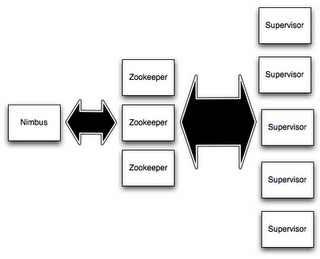
\includegraphics{storm-cluster.png}
        \caption{Các thành phần trong cụm Storm và liên hệ giữa các thành phần}
    \end{center}
\end{figure}

Các thành phần chính của cụm Apache Storm bao gồm: Nimbus, Supervisor, Zookeeper.

Có 2 loại nút trong cụm Storm: nút chủ (master node) và nút thực thi (worker node).

Nút chủ chạy tiến trình "nimbus", chúng chịu trách nhiệm phân phối mã (topology), gán các tác vụ cho các nút worker (Supervisor) và giám sát các lỗi quá trình thực thi của chúng.

Nút thực thi chạy tiến trình "supervisor", chịu trách nhiệm thực thi các phần của topology được gán, chạy hoặc dừng các tiến trình thực thi (worker process) khi cần thiết theo chỉ đạo bởi nút chủ.

Nút Zookeeper, chạy tiến trình "zookeeper", tuy các tiến trình này không được thiết kế dành riêng cho Apache Storm nhưng có vai trò đặc biệt, đóng vai trò điều phối viên giữa Nimbus và Supervisor. Thực tế rằng, cả Nimbus lẫn Supervisor đều là stateless và fail-fast nên có thể ví Zookeeper như trí nhớ của toàn bộ hệ thống. Zookeeper có trách nhiệm lưu trữ thông tin về trạng thái của các nút Nimbus và Supervisor trong cụm Storm. Thông tin này bao gồm trạng thái hoạt động, thông tin cấu hình, và các chi tiết liên quan đến các Topology đang chạy. Thông qua Zookeeper, Nimbus và các Supervisor có thể giao tiếp với nhau một cách dễ dàng, nhất quán, hiệu quả.

Nhờ sử dụng kiến trúc master - slave điển hình đồng thời lưu trữ dữ liệu tại các nút Zookeeper, hệ thống cụm Storm có những ưu điểm tuyệt vời:

\begin{itemize}
    \item Có sự ổn định đáng kinh ngạc.
    \item Trong một cụm, chỉ yêu cầu một nút chủ duy nhất do nút này là stateless (không lưu trữ dữ liệu).
    \item Tương tự như nút chủ, các nút thực thi cũng là stateless giúp tất cả chúng có thể được dễ dàng tái khởi động khi gặp lỗi, sự cố trong quá trình chạy
\end{itemize}

\subsection{Storm rebalance (tái phân bổ Storm topology)}

Trong hệ thống xử lý dữ liệu thời gian thực Apache Storm, một topology (luồng xử lý dữ liệu) được phân bổ và thực thi trên một cluster bao gồm nhiều supervisor node. Sự phân bổ này bao gồm việc gán các worker process và executor thread cho các thành phần (spout và bolt) của topology trên các node có sẵn khi topology được triển khai lần đầu. Tuy nhiên, theo thời gian hoặc do sự thay đổi trong môi trường hoạt động của cluster, như việc thêm hoặc bớt supervisor node, điều chỉnh mức độ song song (parallelism) của các spout/bolt, hoặc khi gặp phải tình trạng mất cân bằng tải giữa các node/worker, cấu hình phân bổ ban đầu có thể không còn tối ưu hoặc phù hợp.

Để giải quyết vấn đề này, Apache Storm cung cấp một tính năng vận hành quan trọng gọi là Rebalance. Về bản chất, Rebalance là quá trình tái phân phối (redistribute) các worker process và executor thread của một topology đang chạy hoặc đã tạm dừng trên các supervisor node có sẵn trong cluster. Mục đích chính của việc thực hiện Rebalance là:

\begin{itemize}
    \item \textbf{Cân bằng tải (Load Balancing)}: Giúp phân phối đều khối lượng công việc và tài nguyên sử dụng trên toàn bộ cluster, tránh tình trạng một số node/worker bị quá tải trong khi các node/worker khác lại nhàn rỗi.
    \item \textbf{Thích ứng với sự thay đổi quy mô (Scaling Adaptation)}: Cho phép topology tận dụng hoặc điều chỉnh theo số lượng supervisor node đã thay đổi trong cluster (ví dụ: sau khi thêm node để tăng năng lực xử lý hoặc bớt node để tiết kiệm tài nguyên).
    \item \textbf{Tối ưu hiệu suất}: Điều chỉnh lại sự phân bổ có thể cải thiện hiệu suất tổng thể và độ trễ xử lý của topology.
    \item \textbf{Phục hồi sau lỗi (trong một số trường hợp)}: Đôi khi Rebalance cũng có thể giúp khắc phục các vấn đề phân bổ phát sinh từ các lỗi không mong muốn.
\end{itemize}

\section{Docker}

Docker\autocite{docker} là một nền tảng mã nguồn mở cho phát triển, phân phối và chạy các ứng dụng. Docker cho phép người dùng tách biệt các ứng dụng của họ khỏi cơ sở hạ tầng giúp công việc phân phối phần mềm nhanh chóng. Với Docker, người dùng có thể quản lý cơ sở hạ tầng theo cùng cách họ quản lý các ứng dụng. Bằng cách tận dụng lợi thế khi áp dụng Docker vào công việc phân phối, kiểm thử và triển khai mã nguồn, người dùng có thể giảm đáng kể thời gian giữa công đoạn viết code với công đoạn triển khai trong thực tế.

\subsection{Nền tảng Docker}

Docker cung cấp khả năng đóng gói và chạy ứng dụng trong môi trường cô lập lỏng lẻo (loosely isolated environment) được gọi là container. Sự cô lập và bảo mật này cho phép người dùng chạy nhiều container đồng thời trên cùng một máy chủ. Các container rất gọn nhẹ nhưng bao gồm đầy đủ các thành phần cần thiết để chạy một ứng dụng, do đó người dùng không cần phải dựa trên các thành phần đã được cài đặt trên máy chủ. Người dùng có thể chia sẻ các container và chắc chắn rằng tất cả những người nhận đều sẽ thu được cùng một container có cách hoạt động y hệt.

Docker cung cấp bộ công cụ và nền tảng để kiểm soát vòng đời của các container.

\begin{itemize}
    \item Phát triển ứng dụng của người dùng và các thành phần phụ trợ sử dụng container.
    \item Các container trở thành đơn vị để phân phối và kiểm thử ứng dụng của người dùng.
    \item Khi người dùng sẵn sàng, triển khai ứng dụng của người dùng trong môi trường kinh doanh, dưới hình thức một container hoặc dịch vụ điều phối (orchestrated service). Tất cả đều có cùng cách hoạt động bất kể là môi trường kinh doanh của người dùng là trung tâm dữ liệu cục bộ, nền tảng điện toán đám mây hay là sự kết hợp của hai môi trường trên.
\end{itemize}

\subsection{Dùng Docker để làm gì?}

\subsubsection{Phân phối ứng dụng một cách nhanh chóng, đồng nhất}

Docker đẩy nhanh vòng đời phát triển bằng cách cho phép các lập trình viên hoạt động trong một môi trường đã được chuẩn hóa sử dụng các container cục bộ - thứ cũng sẽ đồng thời cung cấp các ứng dụng và dịch vụ của bạn. Các container cực kỳ phù hợp với các quy trình CI/CD.

Tất cả các công đoạn trong vòng đời phát triển sản phẩm đều sẽ được tăng tốc thông qua Docker:
\begin{itemize}
    % TODO: Tại sao lại nhanh hơn
    \item Lập trình viên viết mã nguồn và chia sẻ thành quả với các đồng nghiệp sử dụng container của Docker.
    \item Lập trình viên dùng Docker để xây dựng môi trường kiểm thử để chạy các bộ kiểm thử cả tự động lẫn thủ công.
    \item Khi lập trình viên tìm thấy lỗi, họ có thể sửa chúng trong môi trường phát triển rồi tái triển khai chúng lên môi trường kiểm thử để kiểm thử và đánh giá.
    \item Khi hoàn thành kiểm thử, phân phối bản sửa lỗi đến với khách hàng cũng đơn giản như việc triển khai trên môi trường kinh doanh.
\end{itemize}

\subsubsection{Triển khai đáp ứng và co/dãn tài nguyên}

Hiện nay, một sáng kiến có tên The Open Container Initiative (OCI) \autocite{opencontainerinitiative}, được vận hành dưới sự bảo trợ của Linux Foundation \autocite{linuxfoundation} % TODO:
đóng vai trò quan trọng trong hệ sinh thái container hiện đại. Mục đích chính của OCI là phát triển các tiêu chuẩn ngành cho định dạng container và phần mềm thực thi container cho tất cả các nền tảng có sử dụng công nghệ container. Cụ thể là, sáng kiến này sẽ đảm bảo rằng công nghệ container có thể hoạt động đa nền tảng. Điều này có nghĩa là container được xây dựng bởi một bộ công cụ sẽ có thể chạy trên một bộ công cụ khác, giảm thiểu sự phụ thuộc vào nhà cung cấp.

Kết hợp với khả năng tạo môi trường độc lập thống nhất giữa các nền tảng thì các hệ thống được xây dựng dựa trên nền tảng container của Docker hay rộng ra là công nghệ container sẽ cho phép tính di động cao. Hiện nay, các container có thể chạy trên máy tính laptop của lập trình viên, trên máy ảo hoặc máy vật lý trong trung tâm dữ liệu, trên nền tảng điện toán đám mây hoặc là hệ thống kết hợp nhiều mô hình.

Bản chất linh hoạt và gọn nhẹ của Docker còn giúp chúng dễ dàng điều phối khối lượng công việc, tăng/giảm các ứng dụng, dịch vụ nhanh chóng gần như theo thời gian thực.

\subsubsection{Triển khai nhiều khối lượng công việc hơn trên cùng một phần cứng không đổi}

Docker nhẹ và nhanh, có thể coi là một giải pháp thay thế khả thi và tối ưu tài nguyên so với các máy ảo dựa trên công nghệ ảo hóa, nhờ đó người dùng có thể sử dụng tài nguyên hệ thống hiệu quả hơn nhưng vẫn đảm bảo được hiệu suất, khả năng vận hành.

% \subsection{Kiến trúc}
% Docker sử dụng mô hình kiến trúc client-server. Docker client gửi yêu cầu đến Docker daemon, thành phần xử lý toàn bộ các phần việc xây dựng, chạy và phân phối container. Client và daemon có thể chạy trên cùng một máy hoặc kết nối từ xa qua mạng. Chúng giao tiếp qua REST API thông qua socket UNIX hoặc giao diện mạng. Một thành phần quan trọng khác của Docker client là Docker Compose giúp quản lý ứng dụng gồm nhiều container (sẽ được đề cập đến sau đây).

% \begin{figure}[htbp]
%     \centering
%     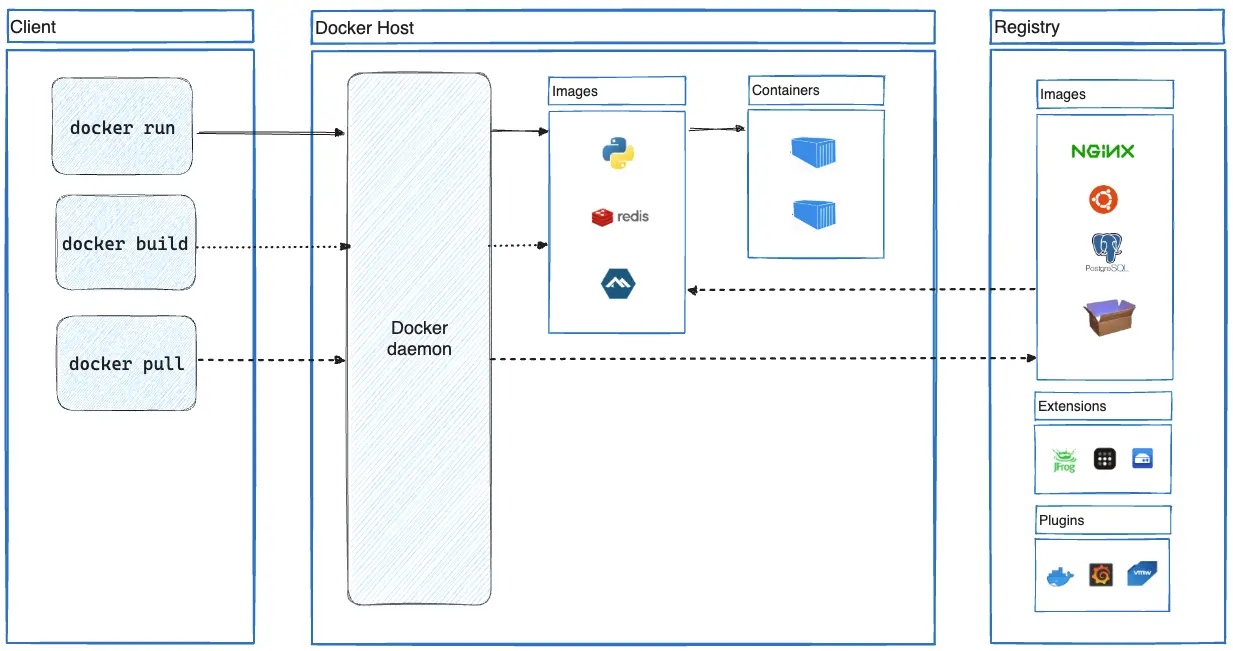
\includegraphics[width=\textwidth]{docker-architecture.png}
%     \caption{Kiến trúc Docker}
% \end{figure}


% \subsubsection{Tiến trình nền của Docker}

% Tiến trình nền của Docker - dockerd lắng nghe các yêu cầu Docker API và quản lý các đối tượng của Docker như image, container, mạng và không gian lưu trữ. Tiến trình nền này có thể tương tác với các tiến trình khác để quản lý các dịch vụ của Docker.

% \subsubsection{Docker client}

% Công cụ dòng lệnh `\texttt{docker}` là phương pháp chính mà người dùng sử dụng để tương tác với Docker. Khi người dùng gửi các lệnh như `\texttt{docker run}`, client sẽ gửi lệnh này đến `\texttt{dockerd}`, tiến trình nền như đã đề cập, sẽ thực hiện các công việc cần thiết để chạy container. Công cụ dòng lệnh `\texttt{docker}` sẽ sử dụng Docker API.

% \subsection{Các đối tượng của Docker}

% \subsubsection{Images}

% Đây là bản hướng dẫn chỉ đọc (read-only template) chứa các hướng dẫn để tạo container. Thông thường một image sẽ dựa trên image khác với một số thay đổi. Có thể sử dụng các image đã được tạo sẵn bởi những người, tổ chức khác đã công bố trên docker registry hoặc người dùng có thể tự xây dựng một bản của riêng.

% Để tạo image của riêng mình, mỗi người dùng có thể tạo tệp Dockerfile với cú pháp đơn giản để định nghĩa các bước cần thiết để tạo image và chạy chúng. Mỗi chỉ dẫn trong Dockerfile tạo thành một lớp trong image. Khi người dùng thay đổi Dockerfile và tái xây dựng image, chỉ các lớp đã bị thay đổi mới bị tái xây dựng. Đây là nguyên nhân khiến cho các image rất nhẹ, nhỏ gọn và nhanh khi so sánh với các công nghệ ảo hóa.

% \subsubsection{Containers}

% Container là thực thể chạy được của image. Người dùng có thể tạo, khởi động, dừng, chuyển, xóa một container thông qua Docker API hoặc CLI. Người dùng có thể kết nối một container với một hoặc nhiều hơn các mạng, gắn các công cụ lưu trữ cho nó hoặc tạo một image mới dựa trên trạng thái hiện tại của container.

% Theo mặc định, một container được phân tách khá độc lập so với các container khác và cả máy chủ đang chạy chúng, tuy nhiên tất cả các yếu tố như mạng của của container, thiết bị lưu trữ hoặc các hệ thống con bên trong đều có thể được tùy chỉnh bởi người dùng.

% Do vậy, các container mở ra khả năng triển khai nhất quán, dễ dàng và hiệu quả trên mọi hạ tầng mà nó được triển khai.

\subsection{Docker Compose}

Docker Compose là một công cụ hỗ trợ định nghĩa và quản lý các ứng dụng đa container một cách dễ dàng. Bằng cách sử dụng tệp cấu hình YAML, người dùng có thể mô tả toàn bộ các dịch vụ của ứng dụng, sau đó triển khai hoặc gỡ bỏ tất cả chỉ với một lệnh duy nhất.

Điểm mạnh nổi bật của Compose là khả năng ghi lại toàn bộ kiến trúc ứng dụng trong một tệp duy nhất, thường đặt tại thư mục gốc của dự án. Điều này không chỉ giúp phiên bản hóa (version control) cấu hình dễ dàng mà còn cho phép người khác đóng góp vào dự án chỉ bằng cách sao chép mã nguồn và khởi động ứng dụng qua Compose. Thực tế, nhiều dự án hiện nay trên GitHub hay GitLab đã áp dụng cách tiếp cận này.

\begin{figure}[htbp]
    \centering
    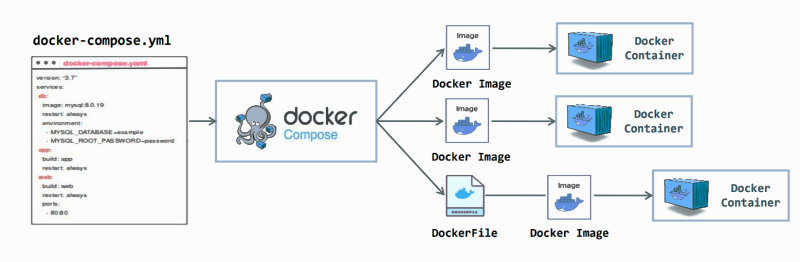
\includegraphics[width=\textwidth]{docker-compose-illustration.png}
    \caption{Minh họa kiến trúc của Docker Compose}
    \footnotesize{Nguồn: https://blog.devops.dev/what-and-why-of-docker-compose-dc95314c74b8, 2025}
\end{figure}

\section{Giám sát hệ thống (monitoring)}

Giám sát hệ thống là quá trình theo dõi liên tục trạng thái và hiệu suất của hạ tầng công nghệ thông tin, bao gồm máy chủ, ứng dụng, mạng và dịch vụ. Mục tiêu chính là phát hiện sớm các bất thường, dự báo sự cố, và đảm bảo hệ thống vận hành ổn định theo thời gian. Hoạt động này thường dựa trên việc thu thập và phân tích các chỉ số như mức sử dụng \gls{cpu}, bộ nhớ, dung lượng đĩa, độ trễ mạng và trạng thái dịch vụ. Khi được triển khai hiệu quả, giám sát hệ thống giúp cải thiện độ tin cậy, tối ưu tài nguyên, và hỗ trợ phản ứng nhanh trước các vấn đề kỹ thuật. Không những vậy, hệ thống này có thể phát hiện các vấn đề tiềm ẩn sớm và khắc phục chúng trước khi có sự cố phát sinh. Đồ án này sẽ sử dụng hai công cụ giám sát hệ thống là Prometheus và Grafana.

\begin{figure}[htbp]
    \centering
    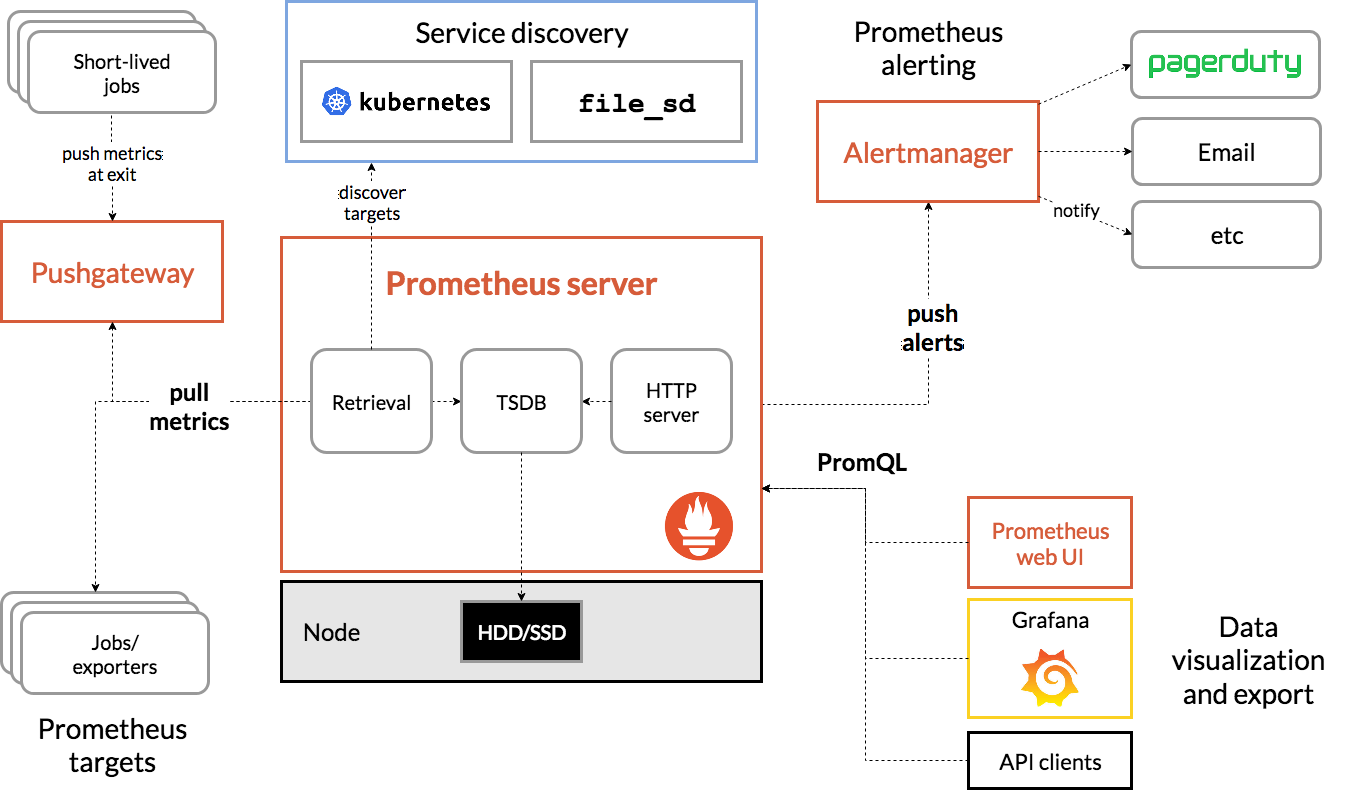
\includegraphics[width=\textwidth]{prometheus-grafana-architect.png}
    \caption{Sơ đồ kiến trúc tổng quan của hệ thống Prometheus và Grafana}
    \footnotesize{Nguồn: https://prometheus.io/docs/introduction/overview/, 2025}
\end{figure}

\subsection{Prometheus}

Prometheus \autocite{prometheus} là một bộ công cụ mã nguồn mở dùng để giám sát hệ thống và cảnh báo, ban đầu được phát triển tại SoundCloud. Kể từ khi ra đời vào năm 2012, Prometheus đã được nhiều tổ chức áp dụng rộng rãi và hiện sở hữu một cộng đồng phát triển và người dùng rất năng động.

Prometheus thu thập và lưu trữ dữ liệu dưới dạng chuỗi thời gian (time series), tức mỗi chỉ số đều được gắn kèm theo dấu thời gian ghi nhận và tập hợp các cặp khóa–giá trị (labels) giúp phân loại thông tin chi tiết hơn.

Các tính năng chính có thể kể đến của Prometheus bao gồm:
\begin{itemize}
    \item Là một mô hình dữ liệu đa chiều với dữ liệu chuỗi thời gian được được định danh bằng tên chỉ số và các cặp khóa/giá trị.
    \item Sử dụng PromQL, ngôn ngữ truy vấn linh hoạt để tận dụng các bản ghi dữ liệu đa chiều.
    \item Tự động phát hiện các mục tiêu thu thập chỉ số thông qua cơ chế khám phá dịch vụ hoặc cấu hình tĩnh.
    \item Thu thập dữ liệu theo mô hình kéo (pull) thông qua giao thức HTTP — một giao thức phổ biến, giúp Prometheus dễ dàng tích hợp với nhiều hệ thống và ứng dụng hiện có.
\end{itemize}

\subsection{Grafana}

Grafana \autocite{redhatgrafana} là một nền tảng mã nguồn mở chuyên về trực quan hóa dữ liệu tương tác, được phát triển bởi Grafana Labs. Công cụ này cho phép người dùng trình bày dữ liệu dưới dạng biểu đồ và đồ thị, gộp lại trong một hoặc nhiều bảng điều khiển (dashboard), từ đó hỗ trợ việc phân tích và hiểu dữ liệu dễ dàng hơn. Từ đó, người dùng có thể hiểu rõ hơn về các mối quan hệ và tương quan giữa các dữ liệu — yếu tố đóng vai trò then chốt trong việc nhanh chóng xác định nguyên nhân gây ra sự cố hoặc các hành vi bất thường trong hệ thống.

\subsubsection{Một số tính năng nổi bật}

\begin{itemize}
    \item Bảng điều khiển (Panels): Cho phép người dùng trực quan hóa dữ liệu theo nhiều hình thức đa dạng như biểu đồ cột, biểu đồ đường, bản đồ địa lý, bản đồ nhiệt,… tùy theo nhu cầu phân tích.
    \item Plugin mở rộng: Cung cấp khả năng hiển thị dữ liệu theo thời gian thực từ nhiều nguồn khác nhau. Người dùng cũng có thể tạo plugin kết nối với API tùy chỉnh để truy xuất dữ liệu đặc thù.
    \item Cảnh báo (Alerts): Một giao diện tập trung giúp cấu hình, tổng hợp và quản lý toàn bộ cảnh báo.
    \item Biến đổi dữ liệu (Transformations): Hỗ trợ các thao tác như đổi tên, tóm tắt, kết hợp, và thực hiện các phép tính trên nhiều nguồn dữ liệu hoặc truy vấn khác nhau.
\end{itemize}

Grafana có khả năng truy vấn dữ liệu và thiết lập cảnh báo từ nhiều nguồn khác nhau như máy chủ truyền thống, cụm Kubernetes hoặc các dịch vụ đám mây. Tuy nhiên, trong khuôn khổ đồ án này, Grafana sẽ chỉ được sử dụng như một công cụ trực quan hóa dữ liệu, với nguồn dữ liệu lấy từ Prometheus, nhằm phục vụ cho việc đánh giá hiệu năng hệ thống một cách trực quan và hiệu quả.

\section{Đám mây công cộng (Public Cloud)}

\begin{figure}[htbp]
    \centering
    
\includegraphics[max width=\textwidth]{global-clou-market.jpeg}
    \caption{Thị phần các nhà cung cấp đám mây công cộng hàng đầu thế giới}
    \footnotesize{Nguồn: https://www.statista.com/, 2025}
\end{figure}

Đám mây công cộng (Public Cloud) là một mô hình điện toán đám mây trong đó các tài nguyên điện toán (như máy chủ, lưu trữ, ứng dụng và dịch vụ) được cung cấp qua internet bởi một nhà cung cấp dịch vụ đám mây (CSP) cho nhiều người dùng.

Đám mây công cộng đóng vai trò then chốt trong các ứng dụng xử lý dữ liệu \gls{iot} bằng cách mang lại nhiều lợi ích vượt trội về khả năng mở rộng, hiệu suất và chi phí. Khả năng mở rộng linh hoạt của đám mây công cộng cho phép dễ dàng điều chỉnh tài nguyên theo nhu cầu dữ liệu IoT, giúp các tổ chức xử lý lượng dữ liệu khổng lồ từ các thiết bị IoT một cách hiệu quả, việc loại bỏ chi phí đầu tư vào cơ sở hạ tầng vật lý giúp tiết kiệm chi phí đáng kể cho các doanh nghiệp. Tốc độ triển khai nhanh chóng của các dịch vụ đám mây cũng giúp dễ dàng triển khai và quản lý các ứng dụng IoT. Ngoài ra, việc sử dụng các công nghệ tiên tiến như AI, máy học và phân tích dữ liệu của nhà cung cấp đám mây giúp các tổ chức khai thác tối đa tiềm năng của dữ liệu IoT để cải thiện hiệu quả hoạt động và tạo ra các dịch vụ mới.

Các nhà cung cấp đám mây công cộng hàng đầu:
\begin{itemize}
    \item Amazon Web Services (\gls{aws})
    \item Microsoft Azure
    \item Google Cloud Platform (GCP)
    \item Viettel Cloud
\end{itemize}

\subsection{Giới thiệu về Google Cloud Platform (GCP)}

Google Cloud Platform (GCP) là một nền tảng điện toán đám mây do Google phát triển, cung cấp một hệ sinh thái phong phú gồm các dịch vụ hạ tầng, nền tảng và phần mềm dưới dạng dịch vụ (\gls{iaas}, \gls{paas} và \gls{saas}). GCP cho phép người dùng xây dựng, triển khai và mở rộng các ứng dụng cũng như dịch vụ thông qua một cơ sở hạ tầng toàn cầu ổn định, bảo mật và hiệu năng cao. Đây chính là nền tảng chạy các sản phẩm cốt lõi của Google như Google Search, Gmail hay YouTube.

GCP bao gồm nhiều dịch vụ quan trọng như:

\begin{itemize}
    \item \textbf{Compute Engine:} cung cấp máy chủ ảo có thể tùy chỉnh cấu hình, hỗ trợ triển khai khối lượng công việc linh hoạt.
    \item \textbf{Google Kubernetes Engine (GKE):} nền tảng quản lý container hiệu quả dựa trên công nghệ mã nguồn mở \acrfull{k8s}.
    \item \textbf{Cloud Storage:} dịch vụ lưu trữ đối tượng có độ bền cao, mở rộng linh hoạt.
    \item \textbf{BigQuery:} hệ thống phân tích dữ liệu lớn (Big Data) với khả năng truy vấn tốc độ cao trên quy mô petabyte.
    \item \textbf{Cloud Run và Cloud Functions:} hỗ trợ triển khai ứng dụng không máy chủ (serverless), phù hợp cho các dịch vụ nhẹ và phản ứng theo sự kiện.
\end{itemize}

Với các tính năng như mở rộng tự động, thanh toán theo mức sử dụng, và tích hợp chặt chẽ với các công cụ học máy (AI/ML), hệ thống giao diện dễ thao tác, chi phí cạnh tranh so với các đối thủ, công cụ GKE có sự tương thích cao với các nền tảng \acrfull{k8s} mã nguồn mở, GCP ngày càng trở thành lựa chọn ưu tiên trong các giải pháp hạ tầng đám mây hiện đại.

\subsubsection{Giới thiệu về Tự động Co dãn trong GCP MIGs}

Nhóm Phiên bản được Quản lý (Managed Instance Groups - \gls{mig}s) của Google Cloud Platform (GCP) cho phép quản lý một nhóm các máy ảo (VM) đồng nhất và cung cấp tính năng tự động co dãn (autoscaling). Tính năng này tự động điều chỉnh số lượng VM trong nhóm dựa trên các tín hiệu như mức sử dụng CPU trung bình, công suất cân bằng tải HTTP(S), chỉ số Cloud Monitoring, hoặc theo lịch trình định sẵn. Hoạt động co dãn luôn bị giới hạn bởi số lượng máy ảo tối thiểu ($minReplicas$) và tối đa ($maxReplicas$) do người dùng cấu hình.

Mặc dù autoscaling trong MIGs mang lại nhiều lợi ích, cơ chế này có những hạn chế nội tại cần được xem xét, đặc biệt là bản chất co dãn bị động (passive scaling) và việc các tham số hoạt động như những giới hạn cứng (hard limits):

\begin{enumerate}
    \item \textbf{Bản chất Bị động - Thiếu Tính Chủ động:} Cơ chế autoscaling của MIG hoạt động hoàn toàn dựa trên việc phản ứng lại các thay đổi của tín hiệu đo lường được (ví dụ: CPU vượt 70\%). Nó không có khả năng chủ động dự đoán xu hướng tải để chuẩn bị tài nguyên trước. Do đó, hệ thống chỉ bắt đầu quá trình scale-out sau khi tình trạng quá tải đã bắt đầu xảy ra, dẫn đến độ trễ và khả năng suy giảm hiệu năng tạm thời trong các đợt tăng tải nhanh hoặc đột ngột. Nó chỉ tuân theo các quy tắc đã được định sẵn một cách máy móc.

    \item \textbf{Giới hạn Cứng $maxReplicas$ Hạn chế Khả năng Đáp ứng Đỉnh Tải:} Trong trường hợp tải tăng vọt bất thường, vượt xa dự kiến, giới hạn cứng $maxReplicas$ sẽ ngăn hệ thống mở rộng thêm, ngay cả khi mọi chỉ số đều cho thấy nhu cầu cấp thiết. Sự kết hợp giữa phản ứng bị động và giới hạn trên cứng nhắc này làm giảm khả năng chống chịu của ứng dụng trước các sự kiện không lường trước.

    \item \textbf{Giới hạn Cứng $minReplicas$ Gây Lãng phí:} Việc đặt $minReplicas$ ở mức cao để đảm bảo tính sẵn sàng có thể gây lãng phí tài nguyên và chi phí trong những giai đoạn tải thấp kéo dài. Do chỉ phản ứng theo quy tắc và bị chặn bởi giới hạn dưới cứng, autoscaler không thể tối ưu chi phí bằng cách giảm số lượng máy ảo xuống dưới mức $minReplicas$ ngay cả khi không cần thiết.

    \item \textbf{Ngưỡng và Quy tắc Cố định Thiếu Linh hoạt:} Các giá trị mục tiêu (ví dụ: target CPU utilization) và các giới hạn $min/maxReplicas$ là các cấu hình tĩnh. Chúng có thể không phải lúc nào cũng tối ưu khi mô hình tải thay đổi. Hệ thống hoạt động theo các quy tắc cố định này và thiếu khả năng tự điều chỉnh các quy tắc đó một cách thông minh dựa trên bối cảnh hoạt động thực tế.
\end{enumerate}

\paragraph{Kết luận}

Tóm lại, cơ chế autoscaling của GCP MIGs là một công cụ mạnh mẽ nhưng hoạt động theo mô hình bị động, dựa trên các quy tắc và giới hạn cứng được định nghĩa trước. Nó không thể co dãn một cách chủ động để đón đầu thay đổi tải. Điều này tạo ra những hạn chế về tốc độ phản ứng, khả năng xử lý đỉnh tải bất thường, tối ưu chi phí và sự linh hoạt trong việc thích ứng với các điều kiện hoạt động đa dạng. Tuy nhiên, đây vẫn có thể được coi như một phương pháp tiềm năng để so sánh hiệu suất với các hệ thống co/dãn trên môi trường điện toán đám mây trong tương lai.


\section{Công cụ quản lý cơ sở hạ tầng Terraform}

Terraform \autocite{terraform} là một công cụ mã nguồn mở mạnh mẽ được phát triển bởi HashiCorp, cho phép người dùng định nghĩa và cung cấp cơ sở hạ tầng dưới dạng mã (Infrastructure as Code - IaC). Thay vì cấu hình tài nguyên một cách thủ công thông qua giao diện người dùng của các nhà cung cấp dịch vụ đám mây, Terraform sử dụng một ngôn ngữ cấu hình khai báo (Declarative Configuration Language) để mô tả trạng thái mong muốn của cơ sở hạ tầng. Điều này mang lại nhiều lợi ích quan trọng, bao gồm khả năng quản lý phiên bản, tái sử dụng cấu hình, và tự động hóa quá trình triển khai và quản lý cơ sở hạ tầng trên nhiều nhà cung cấp dịch vụ đám mây (như \gls{aws}, Azure, Google Cloud Platform) cũng như các hệ thống tại chỗ (on-premises).

Với cách tiếp cận khai báo, người dùng chỉ cần định nghĩa những tài nguyên cần thiết và các thuộc tính của chúng, Terraform sẽ tự động xác định các bước cần thiết để đạt được trạng thái đó. Điều này giúp giảm thiểu sai sót do cấu hình thủ công và tăng tốc quá trình triển khai. Hơn nữa, Terraform duy trì một "trạng thái" (state) để theo dõi các tài nguyên đã được quản lý, cho phép nó thực hiện các thay đổi một cách an toàn và hiệu quả, bao gồm việc tạo mới, cập nhật hoặc xóa bỏ tài nguyên.

Khả năng làm việc với nhiều nhà cung cấp dịch vụ (multi-cloud) là một trong những ưu điểm nổi bật của Terraform. Người dùng có thể quản lý cơ sở hạ tầng phức tạp trải dài trên nhiều nền tảng khác nhau bằng cùng một ngôn ngữ cấu hình và bộ công cụ. Điều này mang lại sự linh hoạt cao và tránh bị khóa chặt vào một nhà cung cấp cụ thể.

Tóm lại, Terraform đóng vai trò là một giải pháp IaC linh hoạt và mạnh mẽ, giúp đơn giản hóa và tự động hóa quá trình quản lý cơ sở hạ tầng, tăng cường tính ổn định, khả năng tái sử dụng và hiệu quả trong việc triển khai và vận hành các ứng dụng và dịch vụ. Việc áp dụng Terraform đã trở thành một xu hướng quan trọng trong lĩnh vực DevOps và quản lý cơ sở hạ tầng hiện đại.

\section*{Các phương pháp mở rộng trong kiến trúc hệ thống}
\label{sec:scaling_comparison} % Gán nhãn để có thể tham chiếu đến mục này

Trong quá trình thiết kế, khả năng mở rộng (scalability) là một trong những yếu tố quan trọng hàng đầu mà chúng ta cần xem xét. Khả năng này đảm bảo rằng hệ thống có thể duy trì hiệu năng, độ trễ thấp và tính sẵn sàng cao ngay cả khi tải làm việc tăng lên đáng kể. Có hai chiến lược chính thường áp dụng để đạt được mục tiêu mở rộng này: mở rộng theo chiều dọc và mở rộng theo chiều ngang.

\paragraph{Mở rộng theo chiều dọc (Vertical Scaling) - Scale Up}

Trước tiên, chúng ta xem xét phương pháp mở rộng theo chiều dọc (Vertical Scaling), còn được gọi là "Scale Up". Phương pháp này tập trung vào việc tăng cường tài nguyên cho một máy chủ hoặc một instance hiện có duy nhất. Điều này có nghĩa là chúng ta sẽ nâng cấp các thành phần phần cứng như CPU, RAM, hoặc dung lượng lưu trữ của máy chủ đó để làm cho nó mạnh mẽ hơn, có khả năng xử lý khối lượng công việc lớn hơn. Về mặt quản lý, mở rộng theo chiều dọc ban đầu thường đơn giản hơn, vì chúng ta chỉ cần quản lý một số lượng hạn chế các đơn vị xử lý có cấu hình cao.

Tuy nhiên, phương pháp này có những hạn chế cố hữu. chúng ta phải đối mặt với giới hạn vật lý về khả năng tối đa mà một máy chủ đơn lẻ có thể đạt được. Hơn nữa, quá trình nâng cấp tài nguyên thường yêu cầu hệ thống phải trải qua một khoảng thời gian chết (downtime), gây gián đoạn dịch vụ. Một nhược điểm nghiêm trọng khác là máy chủ đơn lẻ trở thành điểm lỗi duy nhất (Single Point of Failure); nếu gặp sự cố, toàn bộ dịch vụ có thể ngừng hoạt động, làm giảm tính sẵn sàng và bền bỉ của hệ thống. Chi phí cũng có thể tăng lên đáng kể khi chúng ta đạt đến các cấu hình rất cao.

\paragraph{Mở rộng theo chiều ngang (Horizontal Scaling) - Scale Out}

Tiếp theo, chúng ta phân tích phương pháp mở rộng theo chiều ngang (Horizontal Scaling), hay còn gọi là "Scale Out". Phương pháp này bao gồm việc bổ sung thêm nhiều máy chủ hoặc instance mới vào hệ thống và phân phối, chia sẻ khối lượng công việc giữa các đơn vị này. Thay vì làm cho một đơn vị xử lý mạnh hơn, chúng ta tăng số lượng các đơn vị cùng làm việc song song.

Cách tiếp cận này mang lại khả năng mở rộng gần như không giới hạn về mặt lý thuyết, vì chúng ta có thể tiếp tục gia tăng số lượng máy khi cần, vượt qua giới hạn vật lý của một máy chủ đơn lẻ. Một ưu điểm nổi bật của mở rộng theo chiều ngang là tăng cường đáng kể khả năng chịu lỗi (Fault Tolerance). Nếu một hoặc nhiều máy chủ trong nhóm gặp sự cố, các máy chủ còn lại vẫn có thể tiếp tục hoạt động, đảm bảo tính sẵn sàng và giúp hệ thống phục hồi nhanh chóng sau sự cố. Việc thêm hoặc bớt máy chủ mới thường có thể được thực hiện một cách linh hoạt mà không yêu cầu thời gian chết, đặc biệt khi chúng ta có kiến trúc hệ thống và cơ chế cân bằng tải (load balancing) được thiết kế tốt.

Tuy nhiên, phương pháp này yêu cầu độ phức tạp cao hơn về mặt kiến trúc và quản lý. Trong đó, cần các cơ chế hiệu quả để phân phối tải đến các máy chủ, đồng bộ hóa dữ liệu giữa các đơn vị (nếu ứng dụng có trạng thái), và quản lý một cụm máy lớn hơn. Bản thân các ứng dụng cũng cần được thiết kế để có thể mở rộng ngang một cách hiệu quả, lý tưởng nhất là dưới dạng các thành phần phi trạng thái (stateless) để dễ dàng phân phối yêu cầu.

\paragraph{Thiết kế mở rộng trong hệ thống môi trường điện toán đám mây} Có thể thấy rằng, trong môi trường điện toán đám mây, việc triển khai mở rộng theo chiều ngang sẽ dễ dàng hơn và gây ra ít ảnh hưởng đến hệ thống hơn so với mở rộng theo chiều dọc. Vậy nên, đây sẽ là phương án được sử dụng trong bài đồ án này. Các hướng nghiên cứu tiếp theo có thể phát triển thêm phương án mở rộng theo chiều dọc để gom nhiều instance nhỏ vào thành instance lớn giúp giảm chi phí vận hành và quản lý do số lượng instance giảm và giảm thiểu được số lượng tiến trình nền của supervisor giúp tăng hiệu quả.

\section{Học tăng cường và Q-learning}

\subsection{Học tăng cường}

Học tăng cường (Reinforcement Learning – RL) là một nhánh của học máy, nơi một tác nhân (agent) học cách đưa ra quyết định thông qua tương tác với môi trường. Mục tiêu của tác nhân là tìm ra một chuỗi hành động tối ưu nhằm tối đa hóa phần thưởng tích lũy theo thời gian. Không giống như học có giám sát (supervised learning), học tăng cường không dựa vào cặp dữ liệu đầu vào – đầu ra có sẵn, mà dựa vào cơ chế "thử – sai" (trial and error), nơi tác nhân học từ hậu quả của hành động mình thực hiện.

\begin{figure}
    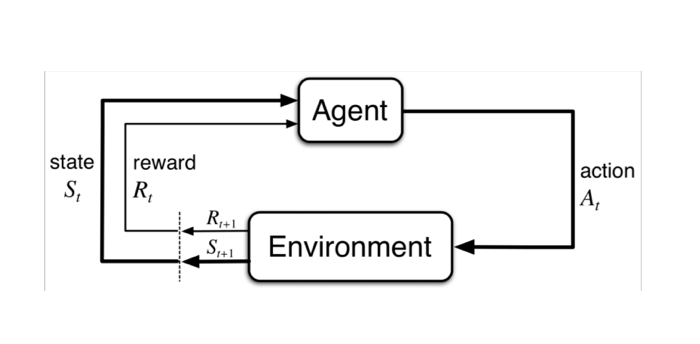
\includegraphics[width=\textwidth]{reinforcement_learning_model.png}
    \caption{Sơ đồ tổng quát mô hình học tăng cường}
\end{figure}

Một mô hình học tăng cường thường bao gồm 5 thành phần cơ bản:
\begin{itemize}
    \item Agent (Tác nhân): Thực thể đưa ra hành động.
    \item Environment (Môi trường): Nơi tác nhân tương tác và nhận phản hồi.
    \item State (Trạng thái): Biểu diễn trạng thái hiện tại của môi trường, bao gồm đầy đủ các thông tin để có thể đưa ra các quyết định.
    \item Action (Hành động): Những gì tác nhân có thể thực hiện.
    \item Reward (Phần thưởng): Phản hồi từ môi trường đánh giá chất lượng của hành động, giúp hướng dẫn tác nhân học.
    \item Chính sách (Policy): Quy tắc quyết định hành động dựa trên trạng thái.
\end{itemize}

\subsubsection{Q-learning}

Q-learning là một thuật toán học tăng cường (Reinforcement Learning) ngoài chính sách (off-policy), nhằm mục đích học một hàm giá trị Q (Q-function) để tìm ra chính sách tối ưu.

Hàm giá trị Q (Q-function) ước tính tổng phần thưởng kỳ vọng khi thực hiện hành động $a$ trong trạng thái $s$ và tiếp tục theo chính sách tối ưu từ đó.

Quá trình cập nhật giá trị Q được thực hiện bằng công thức:

\[
    Q(s, a) \leftarrow Q(s, a) + \alpha \left[ r + \gamma \cdot \max_{a'} Q(s', a') - Q(s, a) \right]
\]

Trong đó:
\begin{itemize}
    \item $s$: trạng thái hiện tại.
    \item $a$: hành động được chọn tại trạng thái $s$.
    \item $r$: phần thưởng nhận được sau khi thực hiện hành động $a$.
    \item $s'$: trạng thái tiếp theo sau khi thực hiện hành động $a$.
    \item $\alpha \in (0,1]$: hệ số học (learning rate), xác định tốc độ cập nhật.
    \item $\gamma \in [0,1]$: hệ số chiết khấu (discount factor), thể hiện tầm quan trọng của phần thưởng tương lai.
    \item $max_a' Q(s', a')$: Giá trị Q lớn nhất trong trạng thái tiếp theo.
\end{itemize}

Nhờ đặc tính không cần biết trước mô hình môi trường, khả năng học từ kinh nghiệm và thích nghi liên tục, Q-learning đặc biệt phù hợp để áp dụng trong các hệ thống co/dãn tài nguyên, nơi mà trạng thái và điều kiện vận hành thường xuyên thay đổi theo thời gian.

\subsubsection{Học Q Sâu (Deep Q-Learning - DQN)}

Học Q (Q-learning) truyền thống sử dụng bảng (tabular Q-learning) để lưu trữ giá trị Q cho mọi cặp trạng thái-hành động $(s, a)$. Tuy nhiên, phương pháp này trở nên bất khả thi khi không gian trạng thái hoặc hành động quá lớn hoặc liên tục, dẫn đến "lời nguyền chiều dữ liệu" (curse of dimensionality). Để giải quyết vấn đề này, người ta sử dụng phương pháp xấp xỉ hàm (function approximation), thay thế bảng Q bằng một mô hình có tham số.

Học Q Sâu (Deep Q-Learning - DQN), được giới thiệu bởi Mnih và cộng sự \cite{Mnih2015HumanlevelCT}, là một phương pháp tiêu biểu sử dụng mạng nơ-ron sâu (Deep Neural Network - DNN) làm bộ xấp xỉ hàm cho hàm giá trị hành động $Q(s, a)$. Mạng này, còn gọi là mạng Q (Q-network), có các tham số (trọng số) $\theta$ và được huấn luyện để ánh xạ một trạng thái đầu vào $s$ tới các giá trị Q ước lượng cho tất cả các hành động khả thi $a$: $Q(s, \cdot ; \theta) \approx Q^*(s, \cdot)$.

Tuy nhiên, việc huấn luyện trực tiếp mạng nơ-ron sâu với dữ liệu từ học tăng cường có thể gặp phải sự mất ổn định do hai vấn đề chính:
\begin{enumerate}
    \item \textbf{Tương quan giữa các mẫu (Correlated Samples):} Dữ liệu $(s_t, a_t, r_t, s_{t+1})$ thu thập theo thời gian có tính tương quan cao, vi phạm giả định về mẫu độc lập và phân phối đồng nhất (i.i.d.) của các thuật toán tối ưu dựa trên gradient như SGD.
    \item \textbf{Mục tiêu không ổn định (Non-stationary Targets):} Giá trị mục tiêu
          \begin{equation}y_t = r_t + \gamma \max_{a'} Q(s_{t+1}, a'; \theta)\end{equation}
          dùng để cập nhật mạng Q lại phụ thuộc vào chính tham số $\theta$ đang thay đổi, làm cho quá trình học trở nên khó hội tụ.
\end{enumerate}

Để giải quyết những thách thức này và ổn định quá trình huấn luyện, DQN đã giới thiệu hai cơ chế đột phá:
\begin{itemize}
    \item \textbf{Bộ nhớ Tái hiện Kinh nghiệm (Experience Replay):} Các chuyển tiếp $(s_t, a_t, r_t, s_{t+1})$ được lưu trữ trong một bộ đệm (replay buffer) $\mathcal{D}$. Thay vì học từ mẫu mới nhất, mạng Q được cập nhật dựa trên các lô nhỏ (mini-batches) gồm các chuyển tiếp được lấy mẫu ngẫu nhiên từ $\mathcal{D}$. Kỹ thuật này giúp phá vỡ tương quan thời gian giữa các mẫu và tăng hiệu quả sử dụng dữ liệu.
    \item \textbf{Mạng Mục tiêu (Target Network):} DQN sử dụng một mạng nơ-ron thứ hai, gọi là mạng mục tiêu, với các tham số $\theta^-$. Tham số $\theta^-$ được sao chép định kỳ từ mạng Q chính ($\theta$) và được giữ cố định trong một khoảng thời gian nhất định. Mạng mục tiêu này được sử dụng để tính giá trị Q cho trạng thái kế tiếp khi xác định giá trị mục tiêu: $y_t = r_t + \gamma \max_{a'} Q(s_{t+1}, a'; \theta^-)$. Việc giữ $\theta^-$ cố định giúp ổn định giá trị mục tiêu, làm cho quá trình huấn luyện hội tụ tốt hơn.
\end{itemize}

Mạng Q chính ($\theta$) được huấn luyện bằng cách tối thiểu hóa hàm mất mát, thường là Sai số Bình phương Trung bình (Mean Squared Error - MSE), giữa giá trị Q dự đoán $Q(s, a; \theta)$ và giá trị mục tiêu $y$ được tính bởi mạng mục tiêu:
$$ L(\theta) = \mathbb{E}_{(s, a, r, s') \sim U(\mathcal{D})} \left[ \left( \underbrace{r + \gamma \max_{a'} Q(s', a'; \theta^-)}_{\text{Giá trị mục tiêu } y} - \underbrace{Q(s, a; \theta)}_{\text{Giá trị dự đoán}} \right)^2 \right] $$
trong đó $\mathbb{E}$ ký hiệu kỳ vọng và việc lấy mẫu $(s, a, r, s') \sim U(\mathcal{D})$ là lấy mẫu ngẫu nhiên đồng nhất từ bộ nhớ tái hiện $\mathcal{D}$. Mục tiêu cuối cùng là tìm được bộ tham số $\theta$ sao cho mạng Q có thể xấp xỉ tốt hàm giá trị hành động tối ưu $Q^*(s, a)$.


\subsubsection{$\epsilon$-greedy}

Trong bài toán học tăng cường, một tác nhân phải thông qua việc lựa chọn các hành động để đạt được phần thưởng tối đa. Với mỗi hành động, ta có hai cách lựa chọn:

\begin{itemize}
    \item \textbf{Exploitation (khai thác)}: chọn hành động tốt nhất đã biết tại thời điểm hiện tại.
    \item \textbf{Exploration (khám phá)}: chọn hành động ngẫu nhiên để khám phá môi trường.
\end{itemize}

Tại sao lại cần cân bằng giữa khám phá và khai thác? Với chiến lược chỉ khai thác, hệ thống sẽ bỏ lỡ những mức phần thưởng cao hơn bị ẩn dấu, có thể mắc kẹt trong cực đại địa phương. Ngược lại với chiến lược chỉ khám phá sẽ không thể tận dụng những hành động tối ưu nhằm tối đa kết quả.

Hiện nay vẫn chưa có nghiên cứu nào xác định được chiến lược tối ưu để cân bằng giữa hai cách lựa chọn. Tuy nhiên chiến lược chọn hành động $\varepsilon$-greedy là thường được cân nhắc như một giải pháp đơn giản nhưng vẫn đảm bảo hiệu quả cân bằng giữa khai thác và khám phá. Trong thuật toán này, tham số $\varepsilon \in [0, 1]$ được sử dụng để điều khiển mức độ khai thác và mức độ khám phá.

Với mỗi lần chọn lựa hành động, ta có thể:

\begin{itemize}
    \item Với tỷ lệ $1 - \varepsilon$ chọn hành động có giá trị Q đạt cực đại tại thời điểm đó - hành động được đánh giá là tốt nhất hiện tại, tương ứng với khai thác - exploitation.
    \item Với xác suất $\varepsilon$ chọn ngẫu nhiên một hành động có trong tất cả các hành động có thể (bao gồm cả giá trị Q cực đại), tương ứng với khám phá - exploration.
\end{itemize}

Tương tự như chiến lược, giá trị tốt nhất của $\varepsilon$ dựa vào bài toán cụ thể chứ không có phương pháp xác định.

Một phiên bản cải tiến của chiến lược này là chiến lược $\varepsilon$ giảm dần, dựa trên thực tế rằng, ban đầu tác nhân có rất ít thông tin về môi trường nên việc khai thác tại giai đoạn này hầu như không có mấy hiệu quả thay vào đó chúng ta cần khám phá trước để xây dựng nền tảng cơ bản. Sau khi có đủ lượng thông tin, lúc này ta sẽ tiến hành khai thác môi trường để tối đa phần thưởng.

Chiến lược $\varepsilon$ giảm dần vẫn sẽ dựa trên chiến lược $\varepsilon$ cơ bản và sử dụng thêm một tham số $\alpha \in [0, 1]$ có vai trò giảm $\varepsilon$ theo thời gian. Vì vậy, $\alpha$ còn được gọi là decay (tạm dịch: độ giảm). Cách lựa chọn hành động vẫn tương tự: khám phá với tỷ lệ $\varepsilon$ và khai thác với tỷ lệ $1 - \varepsilon$. Tuy nhiên sau mỗi hành động, chúng ta giảm $\epsilon$ đi một lượng $\varepsilon * \alpha$, vì lý do này giá trị của $\varepsilon$ khởi đầu sẽ lớn hơn và thường là $\varepsilon = 1.0$ để đảm bảo xác suất khám phá trong giai đoạn đầu sẽ rất cao nhằm nhanh chóng thu được nhiều thông tin nhất có thể về môi trường. Cuối cùng, $\varepsilon$ sẽ giảm về một giá trị $\varepsilon_{min}$ để đảm bảo vẫn có các hành động khám phá trong môi trường nhằm thích ứng khi môi trường biến đổi cũng đồng thời cải thiện thông tin theo thời gian.

\subsection{Thư viện hỗ trợ - Gymnasium}

Trong lĩnh vực học tăng cường (Reinforcement Learning – RL), việc xây dựng và thử nghiệm các thuật toán hiệu quả đòi hỏi sự hỗ trợ từ những môi trường mô phỏng chuẩn hóa. Gymnasium là một thư viện mã nguồn mở, được phát triển như phần kế thừa và mở rộng từ OpenAI Gym, nhằm cung cấp một bộ công cụ thống nhất và linh hoạt để phát triển, đánh giá và so sánh các thuật toán học tăng cường.

Gymnasium cho phép các nhà nghiên cứu dễ dàng tương tác với nhiều loại môi trường khác nhau – từ các bài toán cổ điển như CartPole, MountainCar cho đến các mô phỏng phức tạp trong robotics, game, tài chính, hoặc các môi trường do người dùng tự thiết kế (custom environments). Mỗi môi trường trong Gymnasium đều tuân theo một giao diện chuẩn gồm các hàm cơ bản như reset(), step(action) và các thuộc tính định nghĩa không gian quan sát (observation space) và không gian hành động (action space), từ đó giúp đảm bảo tính tương thích giữa môi trường và thuật toán học.

\chapter{Triển khai của hệ thống Storm SmartHome}

Trong chương này, đồ án sẽ trình bảy triển khai hệ thống xử lý dữ liệu SmartHome xây dựng trên nền tảng Apache Storm trong hai loại môi trường huấn luyện và đánh giá. Tiếp đó là triển khai các chương trình dự đoán tài nguyên và tự động co dãn các máy ảo đa cấp độ trên môi trường điện toán đám mây. Hệ thống được triển khai tại đây sẽ làm cơ sở để đánh giá hiệu quả hệ thống trong và đưa ra kết luận trong các chương tiếp theo.

Trong cả hai giai đoạn đánh giá và huấn luyện đều có cùng các thành phần giống nhau, nội dung chính được trình bày sau đây sẽ đi vào mô tả chi tiết quá trình triển khai và thiết lập của từng thành phần.

\paragraph{Hệ thống tạo dữ liệu của Storm SmartHome}

MQTT publisher được triển khai trên cùng máy chủ với các thành phần của cụm Storm hoặc được triển khai thành máy ảo riêng biệt trong giai đoạn đánh giá. MQTT broker được sử dụng sẽ là broker công cộng EMQX: \href{broker.emqx.io}. Sử dụng broker công cộng sẽ giúp hệ thống mô phỏng tương tác giống với môi trường thực tế hơn khi có độ trễ giữa các gói tin được truyền đi.

Tại thư mục mqtt của bộ nguồn của đồ án \autocite{lemionday_thesis_storm} bao gồm một tệp docker-compose.yml và hai tệp thực thi publish-training.sh và publish-evaluate.sh. Trong đó tệp docker-compose.yml sẽ định nghĩa 6 dịch vụ tương ứng với nguồn phát dữ liệu iot của 6 tòa nhà từ 0 đến 5, tốc độ truyền tin của tất cả các tòa nhà đều được thiết lập là giới hạn 30 gói tin/giấy. Hai tệp thực thi còn lại sẽ định nghĩa các tập dòng lệnh triển khai tương ứng với giai đoạn huấn luyện và đánh giá. Khoảng thời gian giữa mỗi lần thực hiện dòng lệnh là 10 phút nhằm mô phỏng một cách ngẫu nhiên lưu lượng các gói tin thay đổi theo thời gian.

\begin{figure}[H]
    \centering
    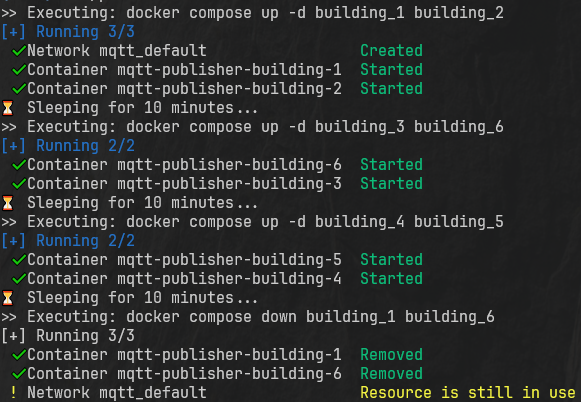
\includegraphics[width=\textwidth]{training-publish.png}
    \caption{Thực thi tệp mô phỏng gửi dữ liệu}
\end{figure}

\section{Hệ thống theo dõi, đánh giá, trực quan hóa dữ liệu}

\paragraph{Storm UI}

Triển khai Storm UI để cung cấp API cho phép Storm exporter thu thập các chỉ số.

\begin{figure}[H]
    \centering
    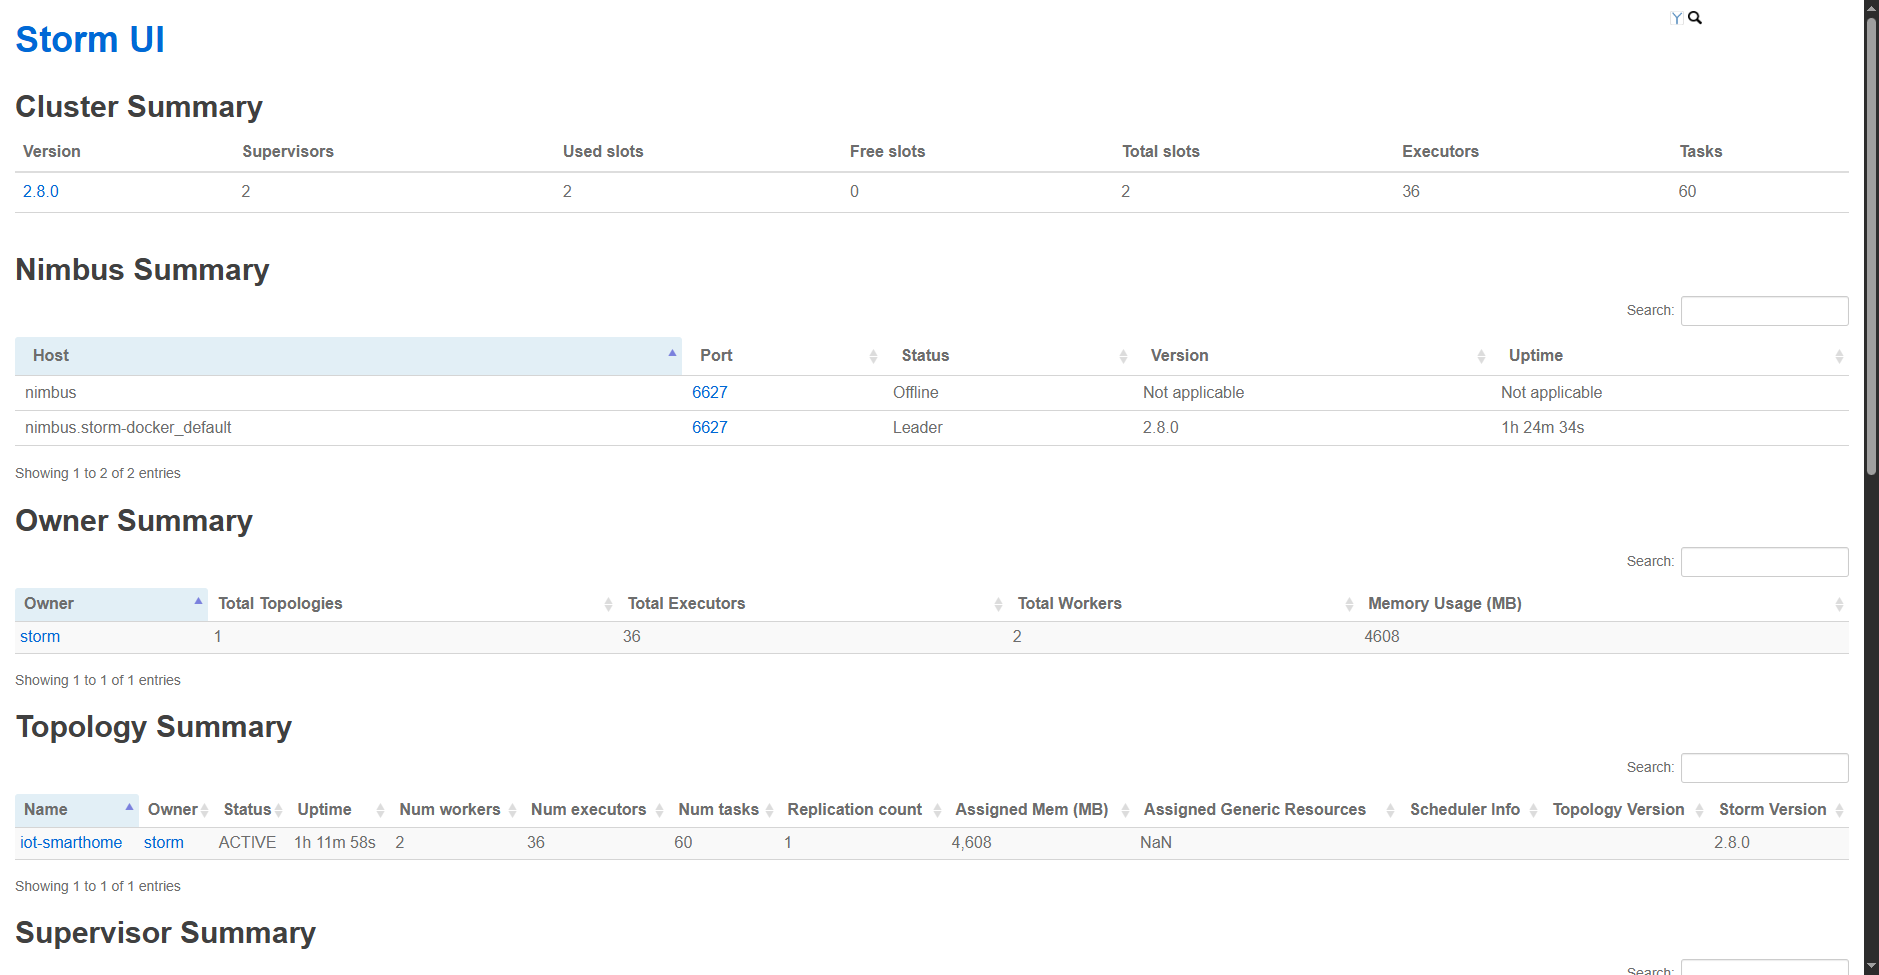
\includegraphics[width=\textwidth]{storm-ui.png}
    \caption{Storm UI}
\end{figure}

\paragraph{Storm Exporter}

Triển khai Storm exporter trên cùng tệp docker compose với storm-ui để thu thập các chỉ số từ topology và supervisor, sử dụng kèm với image socket-proxy \autocite{linuxserver_socket-proxy} để expose Docker socket làm phương tiện giúp Storm exporter đọc dữ liệu trong môi trường huấn luyện thông qua Docker API.

\begin{lstlisting}[language=yaml, caption={Cấu hình triển khai Storm exporter}]
services:
  socket-proxy:
    image: lscr.io/linuxserver/socket-proxy:latest
    container_name: socket-proxy
    environment:
      - CONTAINERS=1
      - EVENTS=1
      - PING=1
      - VERSION=1
    volumes: [/var/run/docker.sock:/var/run/docker.sock:ro]
    restart: unless-stopped
    read_only: true
    tmpfs: [/run]

  storm-exporter:
    build:
      context: .
    container_name: storm-exporter
    restart: always
    environment:
      - STORM_UI_HOST=${STORM_UI_HOST}:${STORM_UI_PORT}
      - REFRESH_INTERVAL=${STORM_EXPORTER_REFRESH_INTERVAL}
      - EXPORTER_LISTEN_ADDR=:${STORM_EXPORTER_PORT}
      - DOCKER_HOST=tcp://socket-proxy:2375
    ports: ['${STORM_EXPORTER_PORT}:${STORM_EXPORTER_PORT}']
    depends_on: [socket-proxy]
\end{lstlisting}

\paragraph{Grafana}
Grafana được triển khai trên máy chủ nội bộ trong cả hai giai đoạn.

\begin{center}
    \begin{figure}[H]
        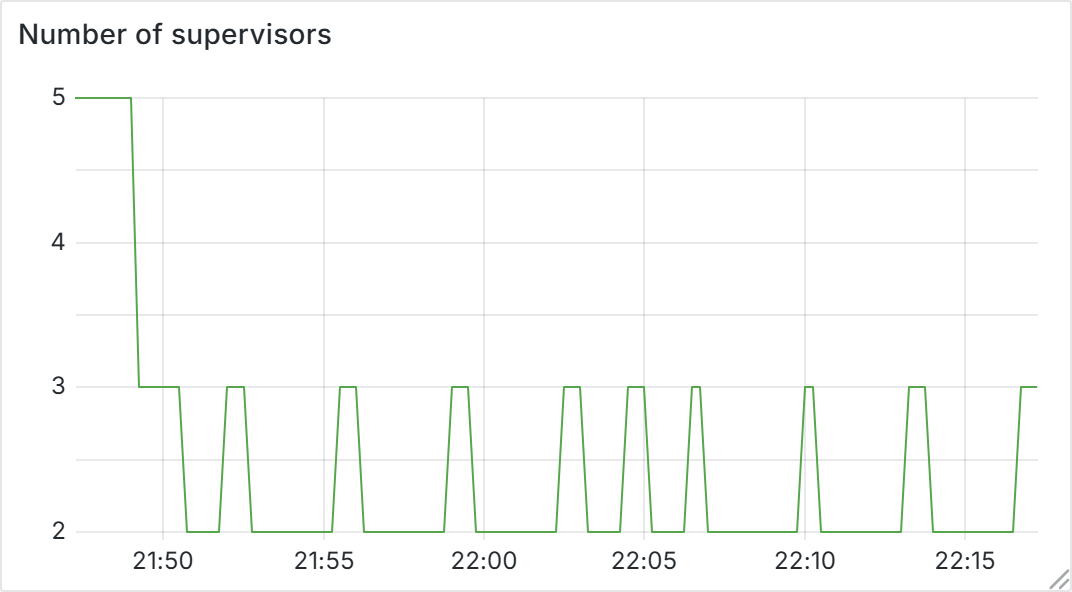
\includegraphics[width=\textwidth]{grafana-number-of-supervisor.png}
        \caption{Theo dõi số lượng supervisor của cụm Apache Storm}
    \end{figure}

    \begin{figure}[H]
        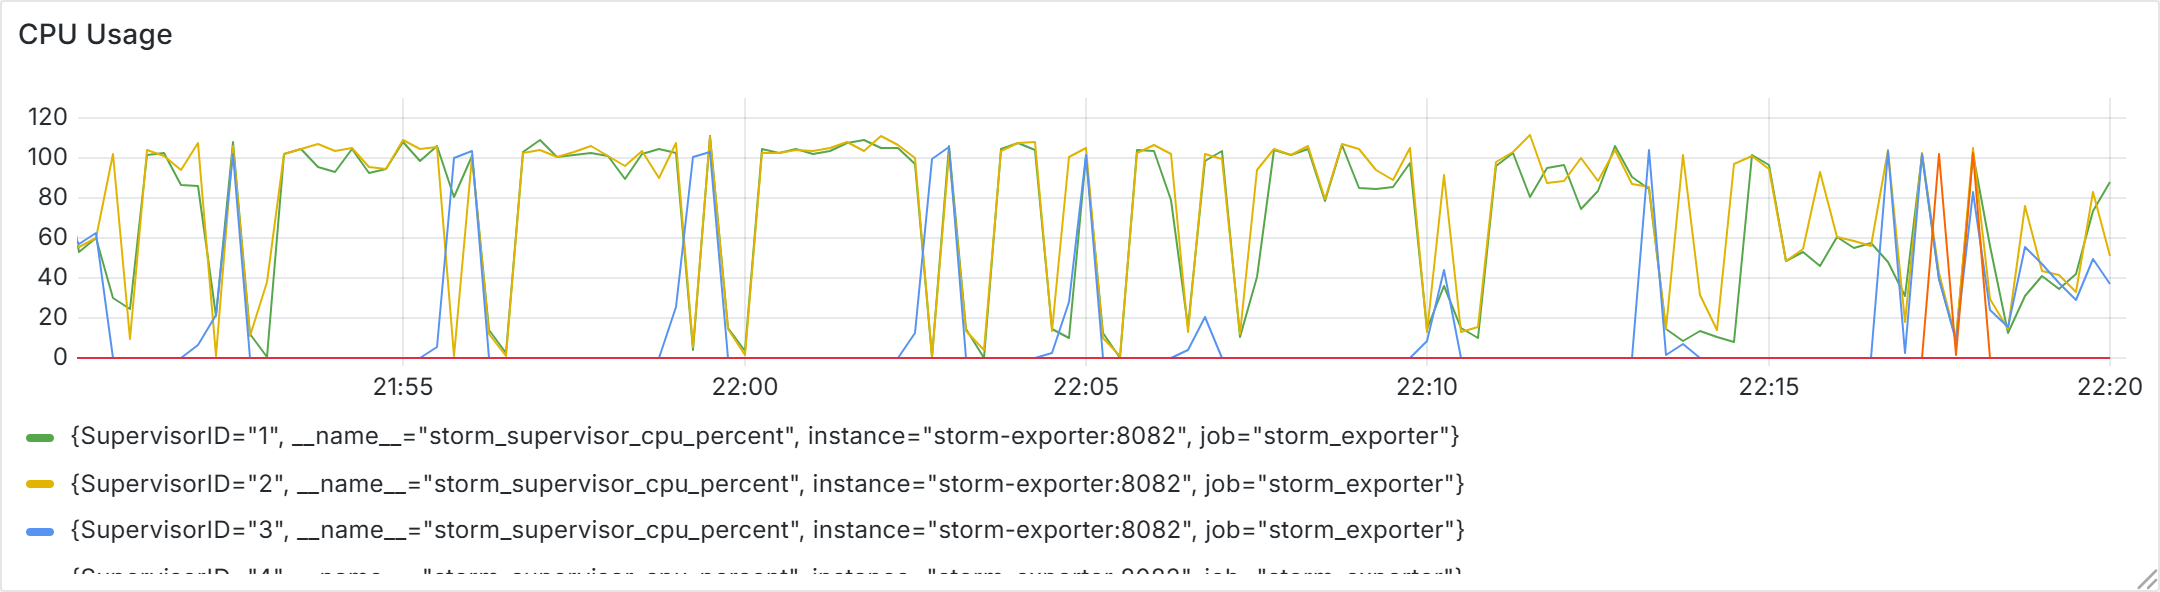
\includegraphics[width=\textwidth]{grafana-cpu-usage.png}
        \caption{Theo dõi tỷ lệ sử dụng CPU của từng supervisor}
    \end{figure}
\end{center}

\section{Hệ thống dự đoán tài nguyên và co/dãn}

Chương trình co/dãn tài nguyên được tác giả viết và lưu trữ trong thư mục autoscaler tại bộ mã nguồn của đồ án \autocite{lemionday_thesis_storm}. Để khởi chạy chương trình, có hai phương pháp

\begin{itemize}
    \item Build và chạy chương trình tại cùng máy chủ với Storm nimbus. Khả dụng cho cả giai đoạn huấn luyện lẫn đánh giá. Lệnh chạy:
          \begin{verbatim}
go build -o build/storm-autoscaler
ENVIRONMENT=Docker build/storm-autoscaler # môi trường huấn luyện
ENVIRONMENT=GCP build/storm-autoscaler # môi trường đánh giá
    \end{verbatim}
    \item Chạy chương trình thông qua image được đóng gói bởi Dockerfile cùng thư mục. Chỉ khả dụng trong giai đoạn đánh giá do không cần tương tác với Docker Compose. Lệnh chạy:
          \begin{verbatim}
docker build --tag storm-autoscaler:v1.0.0 .
docker run -d -e  ENVIRONMENT=Docker storm-autoscaler:v1.0.0
    \end{verbatim}
\end{itemize}

Sau khi triển khai, ta có thể đọc log của Storm autoscaler in ra màn hình.

\begin{figure}[H]
    \centering
    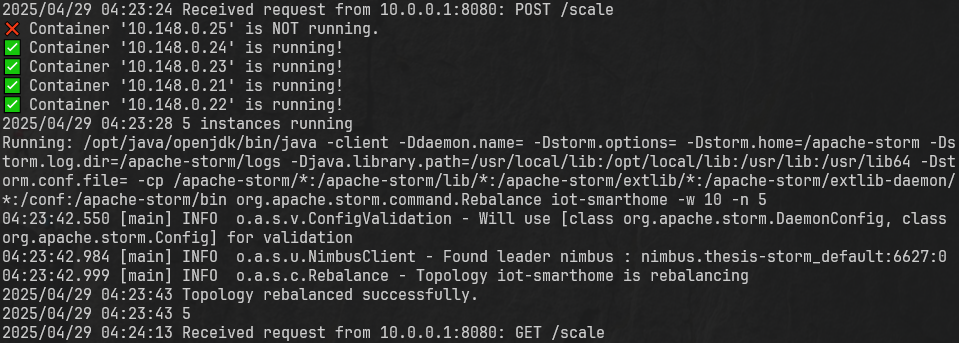
\includegraphics[width=\textwidth]{storm-autoscaler.png}
    \caption{Storm autoscaler}
\end{figure}

\subsection{Giai đoạn huấn luyện}

\begin{figure}[htbp]
    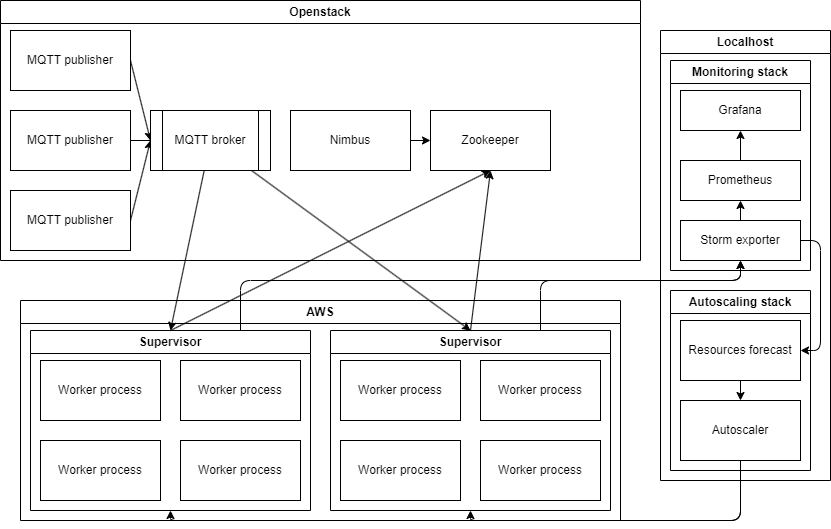
\includegraphics[width=\textwidth]{deployment.png}
    \caption{Sơ đồ triển khai hệ thống trong giai đoạn huấn luyện}
\end{figure}

Giai đoạn này có tác dụng xây dựng và tối ưu hóa bảng giá trị Q cho thuật toán học tăng cường, để hệ thống có thể tiếp xúc, tạo cơ sở về các đánh giá đối với môi trường được mô phỏng, giúp tăng hiệu quả và tốc độ trong giai đoạn sau, giai đoạn đánh giá.

\subsubsection{Triển khai cụm Apache Storm}

Các dịch vụ Nimbus, UI, Zookeeper, Supervisor được chạy trên máy chủ local bằng mô phỏng kiến trúc Docker Compose. Trong đó Storm Supervisor được chạy theo chế độ nhân bản với số lượng tối đa là năm và số lượng tối thiểu là hai. Cấu hình của mỗi Supervisor là 600 MB RAM và 1 vCPU.

\begin{lstlisting}[language=yaml, caption={Cấu hình của các supervisor}]
storm-supervisor:
    image: storm
    restart: always
    command: [storm, supervisor]
    volumes:
    - ./config/hosts:/etc/hosts:ro
    - ./config/storm.yml:/conf/storm.yaml
    deploy:
    replicas: 2
    resources:
        limits:
        memory: 600M
        cpus: 1
\end{lstlisting}

Do tất cả thành phần trên đều kết nối qua bridge network ảo của Docker được đảm bảo độ trễ giữa các dịch vụ không vượt quá 5ms - tương đương với độ trễ trong trung tâm dữ liệu. Mặc dù thành phần gửi dữ liệu (MQTT publisher) và các thành phần của cụm Storm đều nằm trên máy chủ nội bộ, giữa chúng còn có thành phần liên kết là MQTT broker được đặt tách biệt, vậy nên vẫn sẽ có độ trễ giống môi trường thật.Đây có thể coi như mô phỏng khá chính xác giữa môi trường trong giai đoạn huấn luyện với môi trường đánh giá hay thực tế sẽ được triển khai.

\subsubsection{Hệ thống co/dãn tài nguyên}

Docker Compose cung cấp cơ chế chạy các dịch vụ dưới dạng nhân bản (replicas). Dịch vụ trong Docker Compose là một tập các container. Đây sẽ là cơ sở để điều chỉnh số lượng supervisor trong môi trường huấn luyện. Người dùng có thể dễ dàng điều chỉnh số lượng nhân bản của một dịch vụ - cụ thể ở đây là storm-supervisor thông qua lệnh sau:

\begin{verbatim}
docker compose up -d --scale storm-supervisor <number_of_replicas>
\end{verbatim}

Quá trình huấn luyện sẽ được triển khai như đã trình bày tại chương trước, sau khi kết thúc toàn bộ ma trận Q được lưu vào tệp q\_table.npy.

\subsection{Giai đoạn đánh giá}

Giai đoạn này thử nghiệm mô hình trên môi trường điện toán đám mấy để kiểm tra hiệu năng thực tế, tính ổn định và khả năng thích ứng khi tải biến đổi.

\subsubsection{Triển khai máy ảo}

\begin{table}[h]
    \centering
    \resizebox{\textwidth}{!}{%
        \begin{tabular}{|l|l|l|l|l|l|l|}
            \hline
            Máy chủ           & Địa chỉ IP nội bộ    & \begin{tabular}[c]{@{}l@{}}Địa chỉ IP\\ công cộng\end{tabular} & Các dịch vụ chạy           & Cấu hình      & vCPU & \begin{tabular}[c]{@{}l@{}}RAM\\ (GB)\end{tabular} \\ \hline
            storm-manager     & 10.148.0.20          & Có                        & \begin{tabular}[c]{@{}l@{}}Storm Nimbus\\ Storm UI\\ Zookeeper\\ MySQL\\ Prometheus\\ Wireguard\\ Ansible\end{tabular} & e2-standard-2 & 2    & 8                         \\ \hline
            worker{[}0...4{]} & 10.148.0.{[}21-25{]} & Không                     & \begin{tabular}[c]{@{}l@{}}Supervisor\\ Container exporter\end{tabular} & e2-micro      & 2    & 1                         \\ \hline
            forecast          & Không                & Có                        & \begin{tabular}[c]{@{}l@{}}Storm forecast\\ Wireguard\end{tabular} & e2-micro      & 2    & 1                         \\ \hline
            publisher         & 10..148.0.11         & Không                     & MQTT publisher             & e2-micro      & 2    & 1                         \\ \hline
        \end{tabular}%
    }
    \caption{Bảng phân bố các dịch vụ trên các máy chủ GCP}
    \label{tab:gcp-services-distribution}
\end{table}

\begin{table}[h]
    \centering
    \resizebox{\textwidth}{!}{%
        \begin{tabular}{|l|l|l|l|l|}
            \hline
            Máy chủ        & Tên máy chủ   & Vị trí & Vai trò trong Wireguard & Địa chỉ IP Wireguard \\ \hline
            Storm manager  & storm-manager & GCP    & Server                  & 10.0.0.1             \\ \hline
            Storm forecast & forecast      & GCP    & Peer01                  & 10.0.0.2             \\ \hline
            Máy chủ cục bộ & localhost     & Cục bộ & Peer02                  & 10.0.0.3             \\ \hline
        \end{tabular}%
    }
    \caption{Phân bố vai trò và địa chỉ IP của các máy chủ trong VPN Wireguard}
    \label{tab:wireguard-distribution}
\end{table}

\begin{figure}[h]
    \centering
    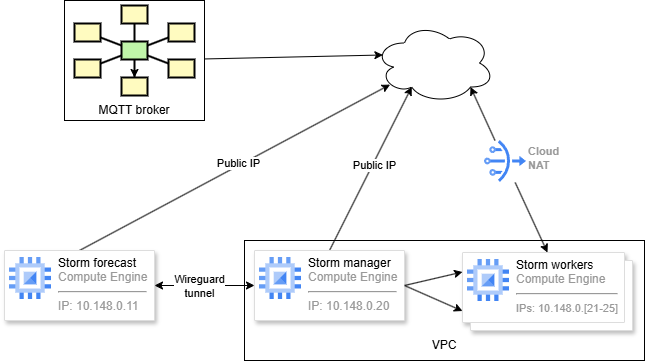
\includegraphics[width=\textwidth]{deployment-GCP.drawio.png}
    \caption{Sơ đồ triển khai GCP}
    \label{fig:deployment-gcp}
\end{figure}

\begin{figure}[h]
    \centering
    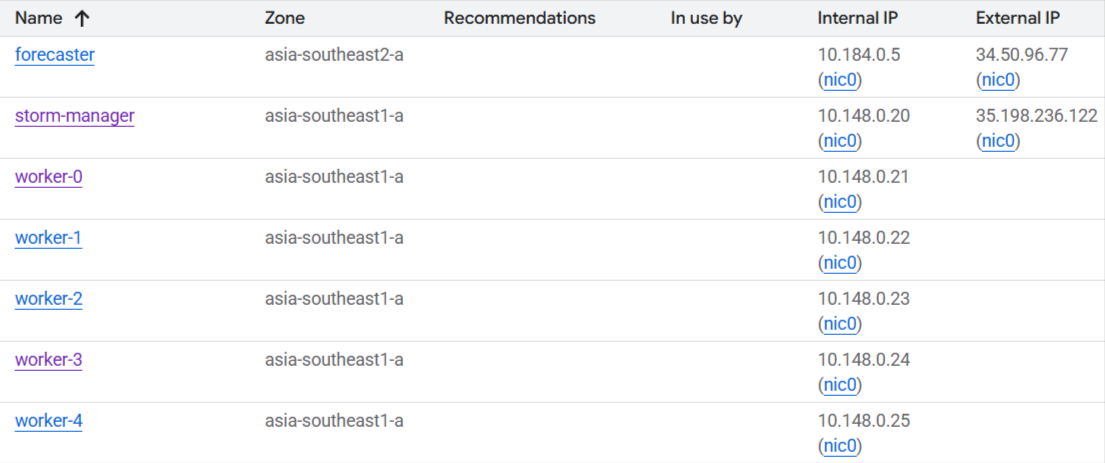
\includegraphics[width=\textwidth]{gcp-compute-engines.png}
    \caption{Khởi tạo máy ảo trên môi trường điện toán đám mây GCP}
\end{figure}

% Please add the following required packages to your document preamble:
% \usepackage{graphicx}
\begin{table}[h]
    \centering
    \resizebox{\textwidth}{!}{%
        \begin{tabular}{|l|l|l|l|l|l|}
            \hline
            Tên              & Nguồn                 & Hướng dữ liệu & Giao thức & Cổng                       & Đối tượng áp dụng          \\ \hline
            allow-ssh        & 0.0.0.0/0             & Vào/ra        & tcp       & 22                         & Tất cả                     \\ \hline
            allow\_wireguard & 0.0.0.0/0             & Vào           & udp       & 51820                      & Tất cả                     \\ \hline
            storm\_firewall  & Dải IP nội bộ của VPC & Vào/ra        & tcp       & \begin{tabular}[c]{@{}l@{}}6627\\ 6628\\ 8000\\ 2181\\ 6700\end{tabular} & \begin{tabular}[c]{@{}l@{}}storm-manager\\ worker-{[}0-4{]}\end{tabular} \\ \hline
            allow\_mysql     & Dải IP nội bộ của VPC & Vào           & tcp       & 3306                       & storm-manager              \\ \hline
        \end{tabular}%
    }
    \caption{Bảng danh sách các quy tắc tường lửa}
    \label{tab:firewall-rules}
\end{table}

Danh sách các máy chủ cùng với địa chỉ IP, cấu hình và các dịch vụ chúng chạy được liệt kê trong bảng \ref{tab:gcp-services-distribution}, sơ đồ thiết kế triển khai được minh họa trong hình \ref{fig:deployment-gcp}. Nhằm nâng cao tính bảo mật đồng thời đơn giản hóa việc áp dụng các quy tắc tường lửa, tác giả đã triển khai thêm hệ thống VPN WireGuard cho Storm manager, Storm forecast cùng với máy chủ cục bộ, cấu hình chi tiết được liệt kê trong bảng \ref{tab:wireguard-distribution}. Đối với các máy ảo trong cùng một VPC của GCP, cụ thể là Storm manager và các worker, việc triển khai WireGuard là không cần thiết do đã có hệ thống tường lửa có sẵn của GCP đồng thời các worker truy cập internet thông qua NAT router của GCP nên khả năng bị tấn công sẽ không có, do vậy ta chỉ cần mở các cổng tường lửa tương ứng với các cổng dịch vụ và thiết lập nguồn gửi trong cùng VPC là có thể đảm bảo hệ thống sẽ hoạt động chính xác. Danh sách các quy tắc tường lửa hệ thống áp dụng đã được liệt kê trong bảng \ref{tab:firewall-rules}.

Quá trình triển khai các máy ảo trên nền tảng GCP được tự động hóa thông qua công cụ Terraform, cho phép khởi tạo đồng thời nhiều máy ảo worker chạy Storm supervisor, dễ dàng điều chỉnh cấu hình và số lượng các worker. Mã nguồn quản lý toàn bộ kiến trúc hạ tầng của đồ án được tác giả viết và lưu trữ trong thư mục cloud của bộ mã nguồn của đồ án \autocite{lemionday_thesis_storm}.

Trong phạm vi luận án này, tác giả đã sử dụng 5 máy ảo worker. Các dịch vụ Storm supervisor được đóng gói và vận hành trong các container trên các máy ảo này, tạo điều kiện thuận lợi cho việc bật/tắt dịch vụ supervisor một cách linh hoạt. Về mặt chi phí, mô hình dự đoán tài nguyên cho phép tác giả cân nhắc việc sử dụng các máy ảo Spot VMs cho một số lượng worker nhất định, tận dụng dung lượng dư thừa của trung tâm dữ liệu trong thời gian thấp điểm để giảm chi phí vận hành máy ảo đến 91\%. Mặt khác, việc đặt chỗ trước (reserved instances) một số lượng máy ảo cũng là một giải pháp tiềm năng để tối ưu hóa chi phí, khi tài nguyên nhàn rỗi trong giai đoạn thấp điểm có thể được sử dụng cho các tác vụ tính toán khác, thay vì chỉ dành riêng cho hệ thống xử lý dữ liệu của ứng dụng SmartHome. Việc kết hợp các chiến lược này có tiềm năng giảm đáng kể tổng chi phí hệ thống.

\begin{lstlisting}[language=HCL, caption={Cấu hình khởi tạo máy ảo worker chạy Storm supervisor}]
resource "google_compute_instance" "worker" {
    count        = 5
    name         = "worker-${count.index}"
    machine_type = var.worker_machine_type
    zone         = var.zone

    boot_disk {
        initialize_params {
        image = "debian-cloud/debian-11"
        }
    }

    network_interface {
        network    = google_compute_network.storm_network.name
        network_ip = var.worker_internal_ips[count.index]
    }

    metadata_startup_script = join("\n",
        [
        file("./scripts/setup_docker.sh"),
        file("./scripts/setup_storm.sh"),
        file("./scripts/setup_storm_supervisor.sh"),
        file("./scripts/setup_docker_exporter.sh")
        ]
    )

    metadata = {
        ssh-keys = "storm:${file("./secrets/storm.pub")}"
    }

    tags = ["storm", "wireguard", "docker-access"]
}
\end{lstlisting}

\paragraph{Cấu hình Nimbus}

Do nền tảng Apache Storm không được thiết kế phù hợp đối với hệ thống co/dãn tài nguyên các supervisor, nguyên nhân là do cơ chế danh sách đen, trong khoảng thời gian dài nếu nimbus không nhận được phản hồi từ các supervisor, chúng sẽ bị đưa vào danh sách đen và phải sau một khoảng thời gian nhất định thì các supervisor này mới có thể được loại bỏ khỏi danh sách đen. Các supervisor ở trong danh sách đen sẽ không được phân phối công việc bởi nimbus, điều này ảnh hưởng rất lớn đến hoạt động của hệ thống khi chúng gây ra hai vấn đề. Vấn đề thứ nhất, số lượng các supervisor được phân phối công việc với số lượng supervisor trong tái cấu trúc (rebalance) không khớp nhau từ đó gây ra thiếu slot cần thiết để thực thi topology, thậm chí có thể khiến hệ thống ngừng xử lý dữ liệu. Vấn đề còn lại, do không được phân phối công việc, supervisor sẽ không có ý nghĩa trong topology, gây lãng phí tài nguyên. Vì lý do này thời gian để các supervisor được loại bỏ khỏi danh sách đen phải đủ ngắn để không bị đưa vào danh sách đen khi được bật trở lại sau khi tắt.

\begin{lstlisting}[language=yaml, caption={Cấu hình Nimbus node}]
storm.zookeeper.servers: [zookeeper]
nimbus.seeds: [nimbus]
ui.port: 8081

supervisor.slots.ports: [6700]

storm.blacklist.scheduler.tolerance.time.secs: 30
blacklist.scheduler.tolerance.time.secs: 30    # window to count failures
blacklist.scheduler.tolerance.count: 1        # failures to trigger exile
blacklist.scheduler.resume.time.secs: 30      # exile duration before return

storm.local.hostname: "nimbus.thesis-storm_default"
\end{lstlisting}

\paragraph{Triển khai ứng dụng xử lý dữ liệu SmartHome lên cụm Apache Storm}

Mã nguồn của topology sử dụng mã nguồn chương trình xử lý dữ liệu nhà thông minh xây dựng trên nền tảng Apache Storm \autocite{fimocodestormsmarthome} với một thay đổi nhỏ là MQTT broker được đổi thành broker.emqx.io. Đầu tiên ta tiến hành đẩy topology đã được biên dịch trên máy chủ cục bộ lên máy ảo storm-manager.

\begin{verbatim}
gcloud compute scp ./stormsmarthome/target/Storm-IOTdata-1.0-SNAPSHOT-jar-with-dependencies.jar storm@storm-manager:~/thesis-storm/stormsmarthome/target   
\end{verbatim}

Sau đó tiến hành triển khai topology tại container nimbus.

\begin{verbatim}
docker exec nimbus storm jar /topologies/Storm-IOTdata-1.0-SNAPSHOT-jar-with-dependencies.jar com.storm.iotdata.MainTopo
\end{verbatim}


\paragraph{Máy ảo supervisor}

Trên mỗi máy ảo supervisor sẽ triển khai hai dịch vụ chính: Container exporter \autocite{shayan_ghani_containerexporter} và Storm supervisor. Trong đó, Container exporter đảm nhiệm việc cung cấp các thông số giám sát hệ thống thông qua đường dẫn \textit{/metrics}, mặc định được lắng nghe tại cổng \textit{8000}. Khác với giai đoạn huấn luyện, khi Storm exporter trực tiếp thu thập dữ liệu từ Docker API của các supervisor cục bộ, trong môi trường triển khai thực tế, nó sẽ thu thập dữ liệu từ đường dẫn \textit{/metrics} của các máy ảo worker. Sau đó, Storm exporter tổng hợp, chuyển đổi tên các metric và bổ sung nhãn để đảm bảo tính thống nhất giữa các môi trường với các truy vấn dữ liệu của hệ thống Storm forecast.

\begin{lstlisting}[language=yaml, caption={Cấu hình các dịch vụ chạy trên máy ảo supervisor}]
services:
    cxp:
        image: devopsteen/cxp:latest
        container_name: container-exporter
        volumes: [/var/run/docker.sock:/var/run/docker.sock]
        ports: [8000:8000]
        environment:
            CONTAINER_EXPORTER_PORT: ${CONTAINER_EXPORTER_PORT}
        restart: always

    storm-supervisor:
        image: storm
        restart: always
        command: [storm, supervisor]
        network_mode: host
        volumes:
        - ./config/hosts.cloud:/etc/hosts:ro
        - ./config/storm.cloud.yml:/conf/storm.yaml
        deploy:
        resources:
            limits:
            memory: 600M
            cpus: 1
\end{lstlisting}

Mỗi supervisor chỉ sử dụng một port duy nhất cho chúng chỉ được cấp 1 CPU, giới hạn bộ nhớ và cpu lần lượt là 600Mb và 100 - tương ứng với 1 CPU.
\begin{lstlisting}[language=yaml, caption={Cấu hình của dịch vụ supervisor}]
storm.zookeeper.servers: [10.148.0.20]
nimbus.seeds: [nimbus.thesis-storm_default]

supervisor.slots.ports:
- 6700

supervisor.memory.capacity.mb: 600
supervisor.cpu.capacity: 100
\end{lstlisting}

\subsection{Triển khai chương trình dự đoán số lượng supervisor - Storm forecast}

Mã nguồn chương trình được tác giả đồ án viết và lưu tại thư mục forecast trong bộ mã nguồn của đồ án \autocite{lemionday_thesis_storm}.

Trong môi trường huấn luyện, lệnh chạy là

\begin{verbatim}
python3 q_learning_agent.py 
\end{verbatim}

Đường dẫn mặc định đến Prometheus là \href{http://localhost:9090}{http://localhost:9090} và đến chương trình autoscaler là \href{http://localhost:8083}{http://localhost:8083}.

Trong môi trường đánh giá, máy ảo storm-manager sẽ chạy dịch vụ wireguard server giúp việc truy cập các dịch vụ trên máy ảo này từ localhost dễ dàng và bảo mật, mặc định địa chỉ của wg0 được gán là 10.0.0.1. Lệnh chạy là

\begin{verbatim}
PROMETHEUS_URL=http://10.0.0.1:9090 \\
AUTOSCALER_URL=http://10.0.0.1:8080 \\
python3 q_learning_agent.py
\end{verbatim}

\begin{figure}[H]
    \centering
    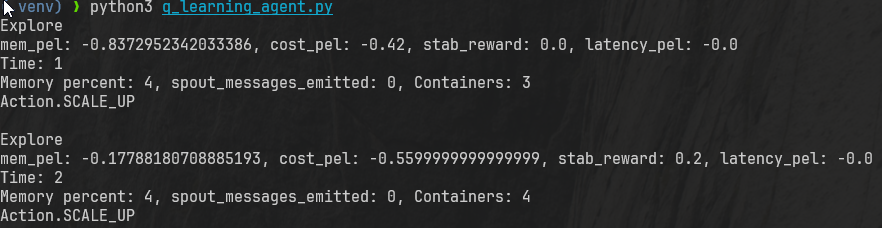
\includegraphics[width=\textwidth]{training-start.png}
    \caption{Bắt đầu quá trình huấn luyện}
\end{figure}

\begin{figure}[H]
    \centering
    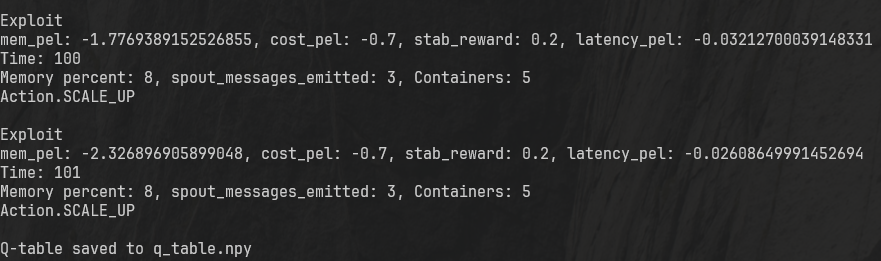
\includegraphics[width=\textwidth]{training-save-q-table.png}
    \caption{Lưu bảng giá trị Q sau khi huấn luyện}
\end{figure}
% \includegraphics[width=0.5\textwidth]{deployment.svg}

% \section{Hệ thống Storm SmartHome}

% \subsection{Hệ thống xử lý dữ liệu lên GCP}
% Hệ thống xử lý dữ liệu bao gồm 4 máy ảo (1 core, 1vCPU) chạy dịch vụ Storm supervisor. Để đơn giản hóa việc triển khai, ta có thể coi việc bật/tắt các dịch vụ Storm supervisor tương đương với việc thêm/xóa các máy ảo chạy dịch vụ Storm supervisor.
% Trên các máy ảo này sẽ được cài thêm chương trình \autocite{prometheus_node_exporter} để thu thập các thông số của máy ảo nhằm cung cấp cho prometheus để đánh giá hiệu năng hệ thống và storm-forecast để dự đoán hệ thống.

% \subsection{Hệ thống theo dõi số liệu}

% \subsubsection{Storm exporter}

% Chương trình lấy từ storm topology các thông số về spout, bolt, topology.

% \subsubsection{Prometheus}

% Thu thập dữ liệu từ storm-exporter, thông số hiệu năng của storm supervisor

% \subsubsection{Grafana}

% Đồ thị hóa các thông số Prometheus thu thập được.

% \subsection{Hệ thống dự đoán tài nguyên}

% \subsubsection{Giai đoạn đào tạo}
% Trong giai đoạn này, chương trình dự đoán tài nguyên được chạy nhiều lần với các thông số đầu vào là thông số hiệu năng của các Storm supervisor, latency trung bình của topology, spout throughput của hệ thống mạng. Từ các thông số đầu vào, tiến hành dự đoán số lượng máy ảo cần sử dụng trong tương lai, dự đoán này được gửi cho chương trình strom-autoscaler để tiến hành điều chỉnh tài nguyên. Sau khi điều chỉnh tài nguyên và tiến hành tái cân bằng (rebalance) hệ thống mạng, các thông số đầu vào được cập nhật để tiến hành đánh giá hiệu quả. Quá trình lặp lại nhiều lần, mỗi lần trong thời gian 10s để tiến đến mô hình huấn luyện tối ưu. Sau khi kết thúc quá trình huấn luyện, mô hình đã được huấn luyện sẽ được lưu lại và sử dụng trong giai đoạn đánh giá. Mục tiêu của dự đoán là giữ spout throughput, latency của topology, cpu và memory usage của máy ảo ở trong ngưỡng bình thường nhưng đồng thời sử dụng số lượng máy ảo là ít nhất.

% \subsubsection{Giai đoạn đánh giá}
% Trong giai đoạn này, dựa trên mô hình đã được huấn luyện, ta tiến hành chạy và đánh giá hiệu quả của chương trình với môi trường của các Storm supervisor là máy ảo trong môi trường AWS.

% \subsection{Hệ thống co dãn Storm-autoscaler}

% \subsubsection{Giai đoạn đào tạo}
% Hệ thống là các máy ảo trong môi trường Openstack

% \subsubsection{Giai đoạn đánh giá}
% Hệ thống là các máy ảo trong môi trường AWS


% \section{Triển khai hệ thống}
% Phần triển khai bao gồm hai giai đoạn chính: \textbf{huấn luyện} và \textbf{đánh giá—triển khai thực tế}. Mỗi giai đoạn được mô tả chi tiết dưới đây.

% \subsection{Giai đoạn huấn luyện (Local)}
% \label{sec:training-local}

% \subsubsection{Mục tiêu và kiến trúc tổng quát}
% Giai đoạn huấn luyện nhằm xây dựng và tối ưu hóa bảng Q (Q-table) cho thuật toán học tăng cường, từ đó hệ thống có khả năng học cách co giãn đa cấp độ chủ động. Mô hình gồm:
% \begin{itemize}
%     \item \textbf{MQTT Broker} và \textbf{MQTT Publisher:}
%           \begin{itemize}
%               \item Broker chạy trên nền OpenStack, không giới hạn băng thông.
%               \item Publisher mô phỏng dữ liệu tải từ 3 tòa nhà (building A, B, C), mỗi tòa nhà phát luồng dữ liệu telemetry về trạng thái CPU, RAM, độ trễ mạng, v.v.
%           \end{itemize}
%     \item \textbf{Apache Storm Cluster:}
%           \begin{itemize}
%               \item \emph{Nimbus}, \emph{UI}, \emph{Zookeeper} khởi động trên máy chủ local.
%               \item 5 node \emph{Supervisor} chạy trên cùng host, mỗi node cấu hình: 700 MB RAM, 1 vCPU.
%               \item Số lượng worker slot động: tối thiểu 2, tối đa 5.
%           \end{itemize}
% \end{itemize}

% \subsubsection{Cấu hình phần cứng và mạng}
% \begin{itemize}
%     \item Tất cả thành phần Local kết nối qua bridge network ảo Docker.
%     \item MQTT Broker và Publisher chạy trên network \texttt{openstack-net}, Storm cluster trên \texttt{local-net}.
%     \item Đảm bảo latency nội bộ dưới 5 ms để phản ánh môi trường trung tâm dữ liệu thực.
% \end{itemize}

% \subsubsection{Chi tiết huấn luyện Reinforcement Learning}
% \paragraph{Đặc tả Môi trường (Environment)}
% \begin{itemize}
%     \item \emph{State} bao gồm: số lượng worker hiện tại, CPU utilization trung bình, queue depth, throughput.
%     \item \emph{Action} là tăng hoặc giảm số worker (±1) trong khoảng [2, 5].
%     \item \emph{Reward} tính theo hàm:
%           \[
%               r = -\alpha \times \text{CPU\_util\%} - \beta \times \text{latency} + \gamma \times \text{throughput},
%           \]
%           với $\alpha, \beta, \gamma$ cân chỉnh để ưu tiên độ trễ thấp và hiệu năng cao \cite{qlearning1967}.
% \end{itemize}

% \paragraph{Thuật toán và siêu tham số}
% \begin{itemize}
%     \item Sử dụng Q-learning $\epsilon$-greedy:
%           \[
%               Q(s,a) \leftarrow Q(s,a) + \eta \bigl(r + \gamma \max_{a'} Q(s',a') - Q(s,a)\bigr).
%           \]
%     \item Hệ số học (learning rate) $\eta = 0.1$, hệ số khấu hao (discount factor) $\gamma = 0.99$.
%     \item Epsilon khởi tạo $\epsilon = 1.0$, giảm dần đến $\epsilon_{min} = 0.05$ trong suốt 10\,000 bước \cite{rlSurvey2020}.
%     \item Số tập huấn luyện (episodes): 5\,000, mỗi episode gồm 100 bước tương tác.
% \end{itemize}

% \paragraph{Quy trình huấn luyện}
% \begin{enumerate}
%     \item Khởi tạo Storm cluster và MQTT môi trường mô phỏng.
%     \item Chạy vòng lặp chính trong một goroutine hoặc thread Python:
%           \begin{itemize}
%               \item Đọc state mới từ bolt xử lý message MQTT.
%               \item Lựa chọn action theo chính sách $\epsilon$-greedy.
%               \item Gửi command thay đổi worker thông qua REST API của Storm.
%               \item Nhận reward và state kế tiếp.
%               \item Cập nhật Q-table.
%           \end{itemize}
%     \item Mỗi 100 episode, lưu checkpoint Q-table xuống local.
%     \item Kết thúc huấn luyện, toàn bộ ma trận Q được lưu vào file \texttt{q\_table.npy}.
% \end{enumerate}

% \subsection{Giai đoạn đánh giá và triển khai (GCP)}
% \label{sec:deployment-gcp}

% \subsubsection{Mục tiêu và tổng quan}
% Chuyển mô hình đã huấn luyện lên môi trường Cloud để kiểm chứng hiệu năng thực tế, tính ổn định và khả năng thích ứng nhanh với biến đổi tải.

% \subsubsection{Mô hình hạ tầng trên GCP}
% \begin{description}
%     \item[Storm Manager VM (e2‑standard‑2):]
%           \begin{itemize}
%               \item Chạy các dịch vụ: Nimbus, Zookeeper, Storm UI, MySQL (lưu lịch sử scale).
%               \item Triển khai \emph{WireGuard Server} để mã hóa và bảo mật liên kết giữa các VM \cite{wireguard2017}.
%               \item Gán \emph{public IP} tĩnh để truy cập UI và quản trị.
%           \end{itemize}

%     \item[Supervisor Nodes (5 × e2‑micro):]
%           \begin{itemize}
%               \item Chạy Storm Supervisor và \texttt{container\_exporter} để thu thập metrics CPU, RAM, I/O \cite{container_exporter2018}.
%               \item Dịch vụ Supervisor được bật/tắt tự động tương ứng với lệnh scale VM.
%               \item Mỗi node có \emph{static internal IP} trong VPC để Storm Manager kết nối ổn định.
%           \end{itemize}

%     \item[MQTT Publisher VM (e2‑micro):]
%           \begin{itemize}
%               \item Chạy script Python mô phỏng 3 tòa nhà, publish lên broker công cộng \texttt{broker.emqx.io} \cite{emqx2021}.
%               \item VM này được gán static internal IP và kết nối ra Internet.
%           \end{itemize}

%     \item[Forecast VM (e2‑micro):]
%           \begin{itemize}
%               \item Chạy WireGuard Client để truy cập private network của Storm Manager.
%               \item Gán public IP để dễ điều khiển và tinh chỉnh tham số trong thời gian chạy.
%           \end{itemize}
% \end{description}

% \subsubsection{Kết nối và bảo mật}
% \begin{itemize}
%     \item Thiết lập VPC riêng, subnet cho Storm và subnet cho MQTT Publisher/Forecast.
%     \item WireGuard kết nối point-to-site từ Forecast và Publisher đến Storm Manager.
%     \item Firewall rules hạn chế chỉ mở port 6627 (Storm Thrift), 8080 (UI), 2181 (Zookeeper), 51820 (WireGuard).
% \end{itemize}

% \subsubsection{Triển khai Q-table và chính sách epsilon}
% \begin{itemize}
%     \item File \texttt{q\_table.npy} được upload lên Storm Manager, bolt khởi động tải vào memory.
%     \item Thiết lập $\epsilon = \epsilon_{min} = 0.05$ để giữ khả năng khám phá nhẹ nhàng trong thực tế, thích ứng với thay đổi về mô tả tải.
% \end{itemize}

% \subsection{Đánh giá hiệu năng và thu thập dữ liệu}
% \label{sec:evaluation}
% \begin{itemize}
%     \item \textbf{Chỉ số đo lường:}
%           \begin{itemize}
%               \item \emph{Response time} trung bình và P95 của hệ thống xử lý dữ liệu.
%               \item \emph{Resource utilization} (CPU, RAM) trên Supervisor nodes.
%               \item \emph{Scale event count}: số lần scale up/down trên mỗi khoảng thời gian.
%           \end{itemize}
%     \item \textbf{Công cụ thu thập:}
%           \begin{itemize}
%               \item Prometheus + Grafana kết hợp với \texttt{container\_exporter} để giám sát real-time.
%               \item Storm UI logs để xác nhận trạng thái topology.
%               \item MySQL lưu lịch sử scale để phân tích bằng Python.
%           \end{itemize}
%     \item \textbf{Quy trình đánh giá:}
%           \begin{enumerate}
%               \item Kích hoạt tải mô phỏng tăng giảm theo kịch bản (peak, off-peak).
%               \item Ghi nhận chỉ số trong 2 giờ liên tục.
%               \item So sánh với baseline (auto-scaling căn bản dựa trên ngưỡng CPU).
%               \item Phân tích kết quả: ưu nhược điểm, thời gian hội tụ, tần suất scale.
%           \end{enumerate}
% \end{itemize}

% In tài liệu tham khảo
\addcontentsline{toc}{chapter}{Tài liệu tham khảo}
\printbibheading[title={Tài liệu tham khảo}]

%\printbibliography[heading=subbibliography, title={Tiếng Việt}, keyword=\textbf{Tieng}, resetnumbers=true]

\DeclareNameAlias{sortname}{family-given}
\DeclareNameAlias{default}{family-given}

\printbibliography[heading=subbibliography, title={Tiếng Anh}, notkeyword=Tieng, resetnumbers=1]
% ===================================================================== %
% CHÚ Ý: phải gán lại resetnumbers=số tài liệu tham khảo tiếng Việt + 1 %
% ===================================================================== %

\end{document}